
\documentclass[MTech]{iitmdiss}

%\usepackage{pifont}
\usepackage{times}
\usepackage{setspace}
\usepackage{amsmath,amsthm,amssymb,amsfonts}
\usepackage{verbatim}
\usepackage{floatrow}
\usepackage{fullpage}
%\usepackage{txfonts,pxfonts,amsfonts}
\usepackage[usenames,dvipsnames]{xcolor}


\usepackage{xcolor}
\usepackage{caption}
\usepackage{subfig}
\usepackage{graphicx}

\usepackage[square]{natbib}
\usepackage[colorlinks=true,linkcolor=blue]{hyperref}
%\usepackage{hyperref} % hyperlinks for references.
\usepackage[all]{hypcap}
\usepackage{complexity}
\usepackage[named]{algo}
\usepackage{algpseudocode}
\newtheorem{thm}{Theorem}
\newtheorem{problem}{Problem}
\newtheorem{corr}{Corollary}
\newtheorem{lma}{Lemma}
\newtheorem{case}{Case}
\newtheorem{rmrk}{Remark}
\newtheorem{prp}{Proposition}
\newtheorem{dfn}{Definition}
\newtheorem{qn}{Question}
\newtheorem{att}{Attempt}
\newtheorem{ex}{Example}
\newtheorem{flaw}{Flaw in Attempt}
% Strut macros for skipping spaces above and below text in tables. 
\def\abovestrut#1{\rule[0in]{0in}{#1}\ignorespaces}
\def\belowstrut#1{\rule[-#1]{0in}{#1}\ignorespaces}

\def\abovespace{\abovestrut{0.20in }}
\def\aroundspace{\abovestrut{0.20in}\belowstrut{0.10in}}
\def\belowspace{\belowstrut{0.10in}}
%%%%%%%%%%%%%%%%%%%%%%%%%


\def\thesistitle{Path Planning in Non-Stationary Environment using RRTs}
\def\thesisauthor{Sai Chaitanya Manchikatla}


\begin{document}
\bibliographystyle{iitm}
%%%%%%%%%%%%%%%%%%%%%%%%%%%%%%%%%%%%%%%%%%%%%%%%%%%%%%%%%%%%%%%%%%%%%% 
% Title page

\title{\thesistitle}

\author{\thesisauthor}

\date{May 2015}
\department{Computer Science and Engineering}

%\nocite{*}
\begin{singlespace}
\maketitle 
\end{singlespace} 

%%%%%%%%%%%%%%%%%%%%%%%%%%%%%%%%%%%%%%%%%%%%%%%%%%%%%%%%%%%%%%%%%%%%%%
% Certificate
\certificate

\vspace*{0.5in}

\noindent This is to certify that the thesis entitled {\bf {\thesistitle}}, 
submitted by {\bf {\thesisauthor}}, to the Indian Institute of Technology, 
Madras, for the award of the degree of {\bf Master of Technology}, 
is a bona fide record of the research work carried out by him under my
supervision. The contents of this thesis, in full or in parts, have not been
submitted to any other Institute or University for the award of any degree or
diploma.

\vspace*{1.4in}
\hspace*{-0.25in}
\begin{singlespace}
\noindent {\bf Ravindran Balaraman} \\
\noindent Research Guide \\ 
\noindent Associate Professor \\
\noindent Dept. of Computer Science and Engineering\\
\noindent IIT-Madras, 600 036 \\
\end{singlespace}
\vspace*{0.20in}
\noindent Place: Chennai\\ 
Date:

%%%%%%%%%%%%%%%%%%%%%%%%%%%%%%%%%%%%%%%%%%%%%%%%%%%%%%%%%%%%%%%%%%%%%%
\acknowledgements
I would like to thank my friends, family for supporting me through out my work. I would also like to extend my gratitude to Ravi sir for his guidance, support and encouragement. 
%%%%%%%%%%%%%%%%%%%%%%%%%%%%%%%%%%%%%%%%%%%%%%%%%%%%%%%%%%%%%%%%%%%%%%
% Abstract

\abstract
Path planning is a widely researched area with applications in diverse fields.  Plainly it involves finding a trajectory through a state space connecting \textit{free configurations} and avoiding collisions with obstacles in the environment. There are many proposed solutions that find a path, if one exists. First we will look at various approaches attempted at tackling path planning under various settings like kino-dynamic constraints, with and without obstacles. We will then present a popular and widely-used sampling based technique known as Rapidly exploring random trees(RRT). There have been many improvements to the vanilla RRT algorithm like growing trees from start and goal states, adding a bias towards goal, etc. We discuss the key advantages and issues with those methods. The performance of RRTs majorly depend on the choice of  distance metric used while computing nearest nodes. Standard metrics like Euclidean would not work in high dimensional domains and choosing a good distance metric is critical for RRTs find a good solution. Even the state of the art algorithms like $RRT^*$ are optimal only in the correct choice of heuristic cost function used in the method. Thus we need a method to find out true cost function or estimate it.

Learning domain dependant metrics through experience was attempted traditionally in Reinforcement Learning(RL). We first present a framework in RL called Markov Decisoin Process(MDP) and ways of solving it. We then present RRTPI algorithm which learns the geodesic distance metric used in RRTs by posing the problem as a MDP. When the environment changes replanning the RRT from scratch is time consuming in complex domains. We will look at various ways of optimizing replanning using RRTs.
We then introduce DYNA, a framework for integrating Planning, Acting, Model-Learning and Direct RL updates. We discuss the how RRTPI behave in dynamic environment and what should be done to find real-time plans in non-stationary environments.
We motivate how DYNA  can be used for solving the issue of path planning in non-stationary environment. We present DYNA-RRTPI algorithm an algorithm responsive to any changes in environment which integrates Planning and Model-Learning in RRTPI algorithm. We demonstrate the use of it in continous state domain in various settings i.e offline vs online and in non-stationary environments. We then present our results in discrete and  continous domains with kino-dynamic constraints.

\pagebreak

%%%%%%%%%%%%%%%%%%%%%%%%%%%%%%%%%%%%%%%%%%%%%%%%%%%%%%%%%%%%%%%%%
% Table of contents etc.

\begin{singlespace}
\tableofcontents
\thispagestyle{empty}

%\listoftables
%\addcontentsline{toc}{chapter}{LIST OF TABLES}
\listoffigures
\addcontentsline{toc}{chapter}{LIST OF FIGURES}
\end{singlespace}

\pagebreak


%The main text will follow from this point so set the page numbering
%to arabic from here on.
\pagenumbering{arabic}
%%%%%%%%%%%%%%%%%%%%%%%%%%%%%%%%%%%%%%%%%%%%%%%%%%
% Introduction.
\input{introduction.tex}
%\input{misc.tex}
%\input{questions.tex}
\chapter{Introduction}

Path planning has become a central problem in robotics since the advent of robots on Industry floors and in daily life. It has impacted both directly and indirectly with applications like robotic surgeries, autonmous self-driving cars, search and rescue operations involving unmanned drones, guided missiles etc. With increasing automation using robots moving autonomously in land, air and water, in previously what were completely human operated jobs path planning has become very much essential part to achieve the robot's goal. Even though different robots vary in sensors, actuators, applications and any other physical differences, the problem of navigation in a complex environment is central to all applications. 

 In its most generic form, Path Planning is the task of finding a valid path in a given configuration space( we will define formally in next chapter). For example, finding out a sequence of steps to be taken to move a robot from initial point to a goal position in a maze is a standard problem tackled in robotics. Other examples include finding out how to move each individual actuators in a robotic arm to take the end gripper from initial position to a required point to grip the object. The problem is not just specific to robotics but is applicable in other domains like computational biology, digital verification. In CAD software where one has to place the components on a chip in a way so that required connections between the components can be made, path planning is used. In animation and gaming industry, various efficient path planning techniques have been implemented to make the games more realistic, and at the same time finding out a path as quick as possible to make the game run on a mobile device with limited resources in real time.
 
  \begin{figure}[htpb]
   \begin{center}
     \resizebox{130mm}{80mm} {\includegraphics *{coc}}
     \caption { Agents moving in a game environment with obstacles. courtesy of supercell games.}
   \label{fig:coc}
   \end{center}
 \end{figure}
 
 
 For example, let us consider the mobile game clash of clans which involves a player’s army trying to take down others village in \ref{fig:coc}. It has various static obstacles like walls, buildings and other dynamic obstacles like troops to defend village as well. A deployed unit should figure out a path to the building to be attacked, navigating through these static and dynamic obstacles. This is a standard problem that occurs in many game settings. Upon close observation one can notice the environment is discretized into grid of cells which are either free to navigate in or consist any obstacles. Each grid cell is connected to 8 surrounding cells. Such problems are relatively easier to tackle. When the search space is smaller and discrete, one can apply Dijkstra’s shortest path algorithm \cite{d59} or A* \cite{hnb68} algorithm to find the path from initial to final points avoiding collisions with obstacles. 
 

 A relatively challenging problem is when the state space is not discrete in the form of grid. For example in \ref{fig:arm} one can see a robotic arm with many joints and gripper at the end in 3-D continuous state space. To take the gripper from one position to desired position, all the joints have to be rotated appropriately. Each joint has constraints on angle it can be rotated. Finding out a sequence of states of angles of each joint to be followed in the \textit{configuration space} to reach the final position avoiding collisions with obstacles in the environment and itself forms the path planning problem. Here one can notice that states are not merely the coordinates of the arm's links in euclidean space but can also contain the information about linkages of the actuators and angle between the actuators.
 
  \begin{figure}[htpb]
   \begin{center}
     \resizebox{130mm}{80mm} {\includegraphics *{arm}}
     \caption { A 6 Degrees of Freedom robotic arm moving in the 3-D surrounding space}
   \label{fig:arm}
   \end{center}
 \end{figure} 
 
 
The path planning problem has been studied for decades now. One can see \cite{choset05}, \cite{deberg00} , \cite{latombe91}  and \cite{lav06} for a detailed introduction to path planning and various attempts at solving the problem. It can be seen that most of the work has been done aimed at stationary environments. In such environments, there would  be no obstacles or if they are present obstacles would be static . Also one can be sure that the environment does not change over time. Hence, one has the advantage of doing a detailed plan once and using it for any future planning requirements. But, in most of the real world scenarios it is rarely the case. Environment changes because of the robot's actions and obstacles are also not fixed. We try and attempt solving the non-stationary environment path planning problem where the world may change over time. We do not treat the obstacles seperately but we model the obstacles also into the environment. For instance, consider a robot doing mapping task in a unknown building. It maps the environment when it enters a room and plans a way to get out of the room. The next time when the robot enters the room some objects might have been moved. Thus earlier plans are valid but necessary modifications have to be made to use them. We deal with such scenarios in which environments are non-stationary but not necessarily moving obstacles whose path can be calculated. Also we try to look at the kinamatic and dynamic constraints on the movement of the robot and try and formulate an algorithm that would generate paths which obey the constraints.

In the next chapter we define the problem of path planning formally and list out different variations of the problem and some approaches that have been tried before. In the further chapters we would detail a sampling based technique to solve path planning called Rapidly Exploring Random Trees(RRTs), followed by our method that uses Reinforcement Learning (RL) techniques for solving the problem optimally. We conclude with experiments in various domains and future work.

\chapter{Path Planning}

One of the earliest breakthroughs in motion planning was the introduction of the concept of configuration space \cite{perez79}.  It made possible to represent any complex shape robot by a single point. Now finding a solution became nothing but finding a path connecting those points in configuration space. 

\section{Configuration space}
  
It allows us to specify the problem. Configuration of a robot in general includes the geometry of the robot, the environment setting and also the geometry of the obstacles. It describes the degrees of freedom the robot has. Configuration space is the set of all such possible configurations of the whole system which includes agent (also referred to as  robot in this work) , the environment and obstacles. It is generally parametrized. For example, the configuration of a robot translating in a 2-D space can be described in terms of 2 parameters x, y. If the robot is allowed to rotate then an additional parameter is required to describe the angle or orientation. The minimal number of such parameter that are required to describe a configuration of the robot are called \textit{degrees of freedom} of the robot. 
In general, there will be these four components in configuration description.

\begin{itemize}
\item Description of the geometry of the moving agent or robot.
\item Description of the geometry of the workspace.
\item Description of robot's degrees of freedom.
\item A start and goal configuration( can be set of configurations also)  for the robot.
\end{itemize}

We denote configuration space by \emph{C} and each parameter in a particular configuration often represents a degree of freedom.
The obstacles, static or moving, does not allow the robot to reach certain configurations. Such configurations which have collisions form the set of forbidden configurations. In case of robotic arm, such forbidden configurations arise not only because of obstacles in the environment but also due to itself, as each joint has limits on the rotating capacity. Let us denote them by \emph{$C_{forbidden}$} or \emph{$C_{obs}$} and rest of the states that can be reached by the robot as \emph{$C_{free}$}. 

\section{The Problem}

A path is a continuous function with its range in the configuration space \emph{C}. It can be defined as follows $$\pi:[0,L] \rightarrow \emph{C}$$  where L is the length of the path. $\pi(0) = s \in C_{free}$ and $\pi(L) = g \in C_{free}$ and $\forall i \in (0,L) \pi(i) \in C_{free} $.The problem of path planning is to find a path between start and goal configurations in configuration space \emph{$C_{free}$}. 
A \emph{complete} path planning algorithm should return the path  between start and goal states in finite time if it exists or it should return failure if such a path does not exist. Also more often than not one would define a cost measure on the path, which can be length of the path or time taken or it can be domain specific. It is used to rank the  paths found. An optimal path is one with the least cost. The problem of finding a solution to path planning is PSPACE-hard \cite{reif79} , where complete planning algorithms( \cite{perez79}, \cite{schsha83},  \cite{canny88} ) exist but are not practically feasible due to their time complexity.  

\section{Related Work}
The path planning problem can be categorised into static and dynamic environments. Further classification can be done based on whether we are operating in known or unknown environment. 
\subsection{Search based algorithms}
For simple cases in a known environment, search based planning algorithms, which discretize the configuration space into grid cells and find the path from start cell to goal cell can be used. A lot of algorithms have been proposed in this genre including Dijsktra's algorithm \cite{d59} which is a best-first search and with introduction of heuristics in algorithms like A*\cite{hnb68} the search space is reduced. These algorithms were even modified to suit dynamic environments in D* \cite{stentz94} which unlike A* algorithm need not be re-run again once environment changes. Also derivates of D* exist which includes Focused D* \cite{stentz95} which addressed the time complexity issues of D*  and quad tree D* \cite{samet88} which reduced the space complexity. Other modern approaches like Anytime A* \cite{hr07}, D*-lite \cite{koeni02} are proposed which reduces the search and time complexity even further.

\subsubsection{Issues}
 But the main limitation of this class of algorithms is that grid is a fixed topology whose resolution must be specified and paths are only optimal at level of  the resolution of the grid. There is always a trade-off between the quality of the path generated and the computational power available. Hence to solve the problems efficiently in known environments other approaches invloving combinatorially computing the explicit paths like Visibility Graph method \cite{visgraph00} and Artificial Potential Field method \cite{khatib86} were introduced.
 
\subsection{Artificial Potential Fields}
Artificial Potential Field method is a practical approach \cite{gecui02} which
 was widely used on many real systems as it relaxed the completeness to \emph{resolution completeness}, which is returning a path if it exists provided that the resolution parameter of the algorithm is set correclty. A potential field is cast in the configuration space where goal applies the attractive force and obstacles apply repulsive force and the robot follows the steepest descent in the resulting potential field to reach the destination. But this has the issue that robot might get stuck in points of local optima. There were proposed solutions \cite{barra91} to tackle this  but it does not apply to all problems in general. ARF is particularly suited for applications where translation is any direction is major degree of freedom as one calculates the potential of a point based on the distance from the source in the workspace or configuration space. 
\subsubsection{Issues}
 One can notice that it requires explicit representation of the obstacles in the configuration space which is not always the case in many real world tasks. Also even if they are explicitly mentioned, presence of large number of obstacles would give rise to lot of computational overhead as solution is built directly using explicit representation of obstacles  in state space . Hence only low dimensional C-spaces and simplified geometries have been solved efficiently using these methods. Avoiding such explicit representation was done in the next set of algorithms known as sampling based algorithms. These algorithms were ideally suited for unknown or partially known environments as they do not ask for explicit representation of the obstacles in the configuration space.
 
\subsection{Sampling based planners}
In the sampling based motion planners, the configurations in \emph{$C_{obs}$} are determined just by sampling C-space using \emph{collision detectors}, which would tell us whether a given configuration is a part of $C_{free}$ or $C_{obs}$. Thus the modern collision detection algorithms keep track of simple metrics like distance between robot and obstacles in the environment to specify that. It makes even complicated models to be specified and solved efficiently using limited information about the configuration space. There is no need to enumerate all possible contact cases of our robot and obstacles nor compute the contact cases to solve for a trajectory. Also it makes the problem simpler as the collision detection can be treated as separate module. The simplicity and genarality made the sampling based planners to be successfully applicable to wide range of motion planning problems even with high dimensional configuration spaces. For a full historical evolution of sampling based
 planners one may look into \cite{linde05}. One of the highly used sampling-based planners was Probabilistic Road Map method \cite{kavraki96}. 
 
\subsubsection{Probabilistic RoadMap}
The most basic implementation, Probabilistic RoadMap is very simple and works in two phases. In the preprocessing phase the algorithm builds a road map( a graph $G(V,E)$ )  by attempting to connect points sampled from $C_{free} $. In the query phase it uses the roadmap to query for paths . Algorithm begins with an empty graph. In preprocessing phase it samples a point $x_{rand}$ from the state space and if it falls in $C_{free}$ it is added to vertex set \emph{V}. Then it attempts to connect all points that are in r-radius sphere from the $x_{rand}$ in the order of incresing distance from $x_{rand}$ i.e nearest first using a simple local planner. The local planner checks if a path is possible by checking collisions with any obstacles. If there are no collisions then the points are added to the graph by joining edges between the point and $x_{rand}$. For sake of simplicity the connections are only added if the randomly sampled point is not connected to any connected components of the new point. This prevents any formation of cycles, resulting in a forest ( set of trees ). There are other simpler modifications, where initially the algorithm samples 'n' points in the space and further it form trees among those 'n' points only. In other work \cite{lav06}
 the selection of vertices has been modified from r-radius disc to k-nearest neighbours of the randomly sampled point. This forms a k-nearest graph. There were other modifications involving setting bounds on the number of vertices picked from the r-radius disc. Other ways of modifying the algorithm is to have a variable radius disc from which one tries to join points to the randomly sampled point. These versions are called k-Nearest PRM, bounded degree PRM, and variable radius PRM respectively. If a roadmap was constructed for a particular configuration, it can be used to query for paths between any pairs of configurations in the environment in the Query phase. To implement this, we connect the two query configurations to the existing roadmap and treat them like new nodes inserted into the roadmap during the previously described construction phase. If it succeeds a path is searched for in the roadmap. It is usually the case that paths generated from Probabilistic Roadmap technique have to undergo some post processing to give smooth paths. Other variants of PRMs differ in the choice when joining two configurations using the local planner. In the simplest case we used a straight line. Also how we determine the neighbors, to which connection is attempted can be varied. Local planners can be made to try complicated connections and ways of choosing the points to attempt connections to. One can choose all points in the neighbouring set but that takes time. One can choose to attempt to only k-nearest neighbours within a bounded distance $d_{max}$. Such things take time because of hefty computations. In some scenarioes, one cannot afford time on such steps. Thus one has to be careful in making a tradeoff between the real-time application of the planner vs the complexity we need. PRMs are not complete i.e., if a valid path does not exist between the start and end points in $C_{free}$, they would not be able to notify that. However, it is to be noted that PRMs are probabilistically complete. If there exists a path between start and goal configurations in $C_{free}$, then the probability that PRM-roadmap contains a solution tends to 1 as the roadmap creation time tends to infinity
 \cite{kavraki98}
 Creating a roadmap takes lot of time and once it is created all future queries can make use of this prepossessing step to fetch results faster. Such problems are called multiple query problems. In contrast to this, when there is only one valid query to be made in a given setting it is called single-shot method. Frazzoli et al 
\cite{karaman11} 
 proposed PRM*, an optimal version of the PRM where they limit the number of points in the neighbourhood to extend to either by setting bound on k in the k-nn approach or by setting the radius of the disc. 

\subsubsection*{Issues}
 This is of importance in fast and changing environments where the roadmap created might not be valid for future queries. Hence in dynamic environments, various techniques like single-query PRMs were introduced but the most successful and widely used algoritms for their simplicity are Rapidly Exploring Random Trees. We discuss RRTs and modifications to basic algorithm in the next section.  

\chapter{Rapidly Exploring Random Trees}

RRT is a single shot sampling based algorithm. In the basic version the algorithm incrementally builds a tree of feasible trajectories with the start point as root node. The algorithm then samples a point $x_{rand}$ randomly in the space. It then tries to connect the point to the already existing tree by movin the \emph{nearest} point $x_{near}$ in the tree using a local planner towards the sampled point. The local planner adds an edge to the tree if the path is not colliding with any obstacle. To mininize the collisions the algorithm instead of joining $x_{rand}$, it tries to move from $x_{near}$ in the direction of $x_{rand}$ by a small $\epsilon$-distance or moving in that direction for a small $\delta$-time using the local planner, resulting in a new point $x_{new}$. We would later on see the other implications of this formulation in the kino-dynamic setting. If there are no collisions in joining $x_{near}$ and $x_{new}$ an edge is added between them and algorithm proceeds to pick another point. It is shown in \ref{fig:rrt-extend} This continues until the goal is reached or maximum points are drawn . An RRT grown in 2-D continuous space from the start state (50,50) can be seen in \ref{fig:rrt-basic}.

  \begin{figure}[htpb]
   \begin{center}
   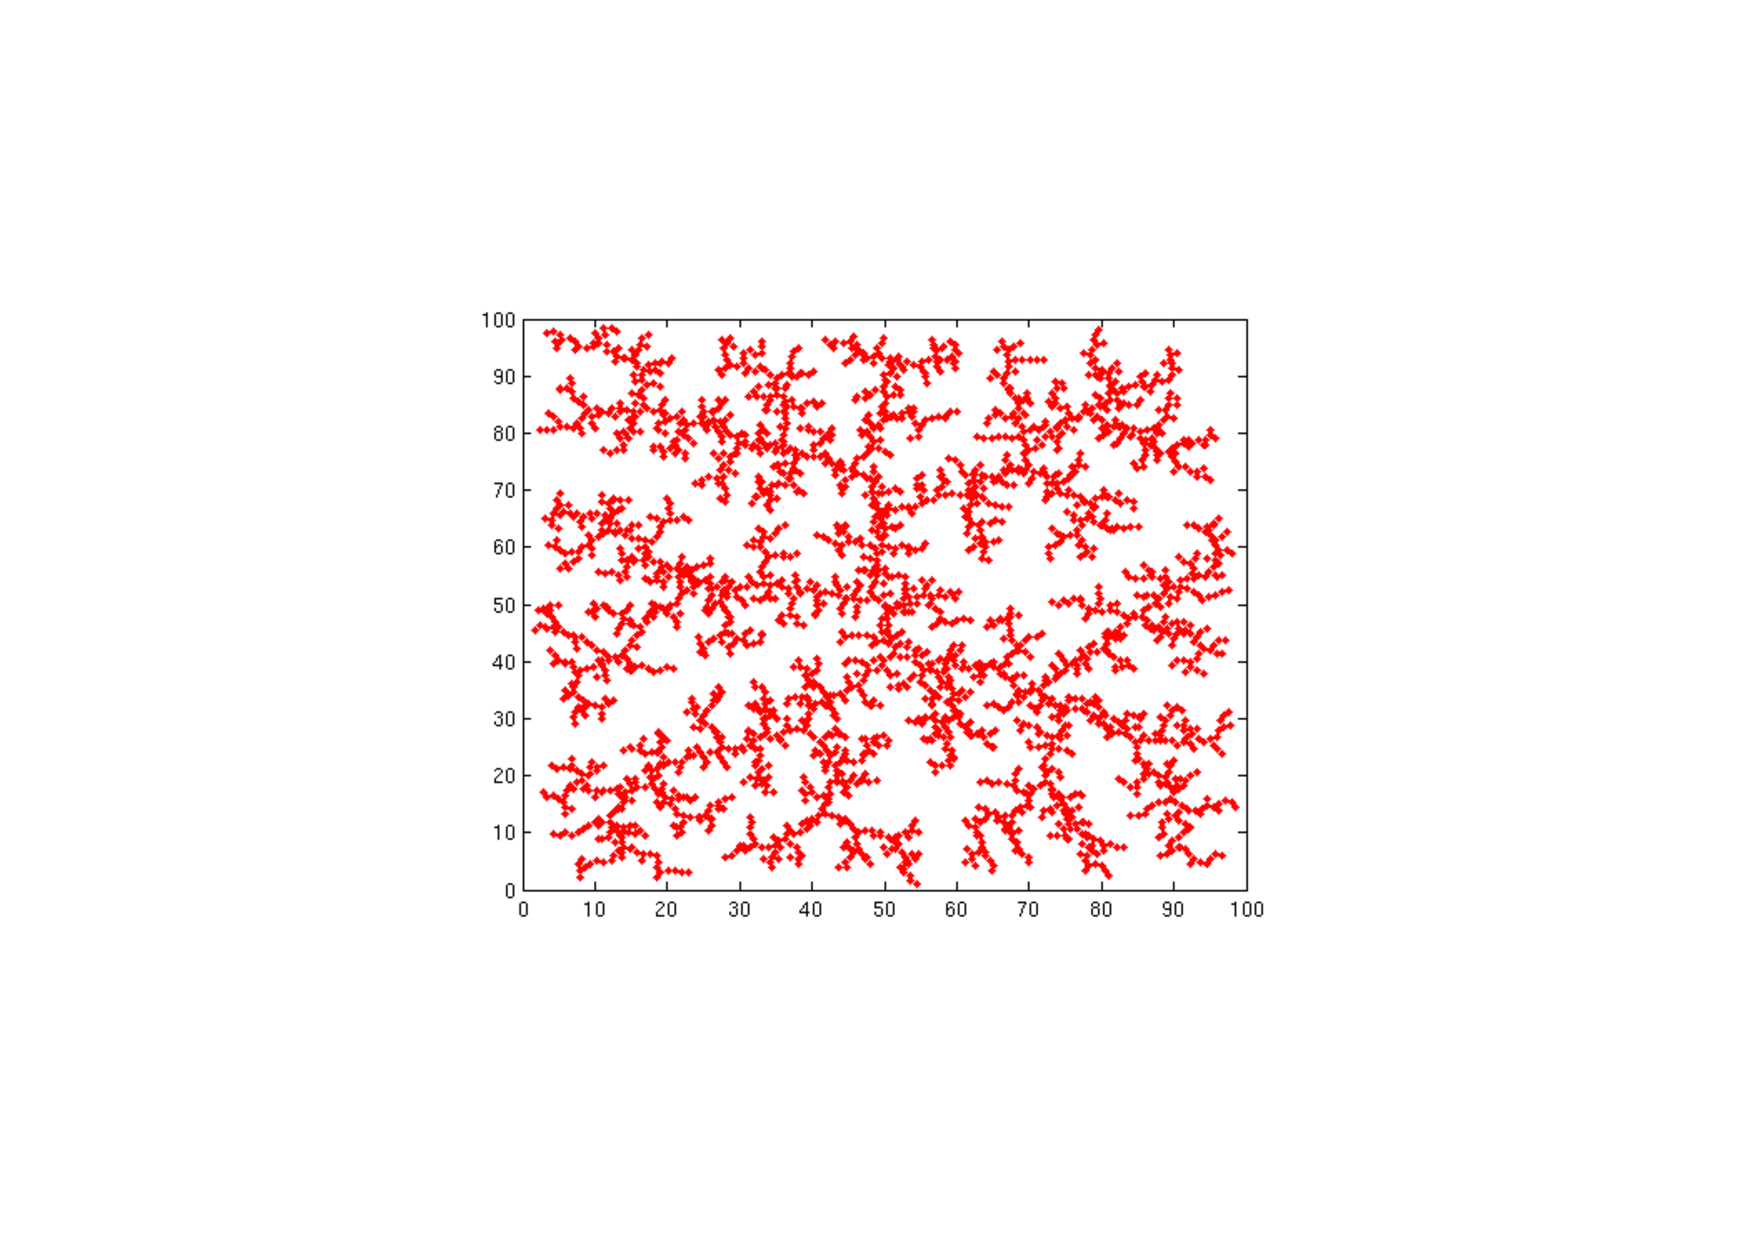
\includegraphics[scale=0.45] {rrt-basic}
%     \resizebox{80mm}{80mm} {\includegraphics *{rrt-basic}}
     \caption { A RRT grown from start point [50;50]. It explores the whole state space due to the space filling property.}
   \label{fig:rrt-basic}
   \end{center}
 \end{figure}

The probability of \emph{extending} a point in the tree is directly proportional to the \emph{voronoi} region of the point. A voronoi region of a point is all the set of points in the space to which it is the nearest neighbour. Thus RRTs have excellent space filling properties. This accounts for the \emph{rapidly-exploring} aspect of the RRTs. The tree is thus streched towards the lesser explored regions of the state space. If a big area is unexplored then the probability that the RRT will extent towards that region is higher than other regions. RRTs are shown to be probabilistically complete. The probability of finiding a solution if it exists tends to 1 as the number of samples picked tends to infinity. RRTs have been successfully implemented in many domains as seen in \cite{lav01, bruce02, kuffner03, kim03, oriolo04}

\section{Algorithm}
 \begin{figure}[htpb]
   \begin{center}
     \resizebox{75mm}{75mm} {\includegraphics *{rrt}}
     \caption {Process of building the RRT and extending the current tree to $x_rand$}
   \label{fig:rrt-extend}
   \end{center}
 \end{figure}

\begin{algorithm}{Build-RRT}{
\label{algo:Build-RRT}
\qcomment{builds an RRT in a state space}}
 V(G) $\leftarrow$ {$x_{start}$};  E(G) $\leftarrow${$\phi$ } \\
\qwhile goal is not reached \\
$x_{rand}$ $\leftarrow$ Sample(S);\\
$x_{near}$ $\leftarrow$ Nearest($x_{rand}$, V(G));\\
$x_{new}$ $\leftarrow$ Extend($x_{near}$, $x_{rand}$, S);\\
\qif Not-Colliding($x_{new}$, $x_{near}$,S)\\
\qthen Connect $x_{new}$ to $x_{near}$\qfi \qend\\
End of Algorithm
\end{algorithm}

\begin{algorithm}{Nearest($x_{rand}$, V(G))}{
\label{algo:Nearest}
\qcomment{Finds a point nearest to given point in the graph}}
return the vertex that minimises $||v - x_{rand} ||$, where $||$ x-y  $||$ is the euclidean norm\\
End of Algorithm
\end{algorithm}

\begin{algorithm}{Extend($x_{near}$, $x_{rand}$, S)}{
\label{algo:Extend}
\qcomment{Finds a point close to $x_{rand}$ that is in $\epsilon-$neighbourhood of $x_{near}$}}
return a point $x_{new}$ $\in$ $S$ such that $||x_{near} - x_{new} ||$ $<$ $\epsilon$ which minimises $||x_{new} - x_{rand} ||$ \\
End of Algorithm
\end{algorithm}

\section{Improvements}
Thus RRTs incrementally build a tree sampling points from the state space. If the state space is large it takes long times to find the path to goal. Hence a little bias is added towards goal to direct the exploration making it faster. It is incorporated in the sample function as seen in line 3 of the \ref{algo:Bias-Sample}

\begin{algorithm}{Bias-Sample(S)}{
\label{algo:Bias-Sample}
\qcomment{Samples a point $x_{rand}$ in the state space S}}
prob $\leftarrow$ Random(0,1)\\
\qif prob $<$ $p_{goal}$\\
\qthen $x_{result}$ $\leftarrow$ $x_{goal}$\\
\qelse $x_{result}$ $\leftarrow$ Randomly sample a point from the state space \qfi\\
return $x_{result}$\\
End of Algorithm
\end{algorithm}

 \begin{figure}[htpb]
   \begin{center}
     \resizebox{150mm}{70mm} {\includegraphics *{rrtnobias}}
     \resizebox{150mm}{70mm} {\includegraphics *{rrtbias01}}
     \resizebox{150mm}{70mm} {\includegraphics *{rrtbias02}}
     \caption {A snapshot of growth of RRT starting at [50;50] and goal at [95;95]the first column is at 200 samples and second column at 2000 samples.The first row is taken when sampling randomly , second row at 10 percentage bias to goal and third row at 20 percentage  bias towards goal }
   \label{fig:rrt-bias}
   \end{center}
 \end{figure}
 
Other ways in which people have looked speeden up the process is to grow multiple trees towards a region and connect them. One approach was called RRT-Connect
\cite{kuffner00}
 This algorithm keeps track of two trees one from the start and other from the goal states. Initially one tree is begun from start state and it is extended by a small step towards a random point to reach a target point which is then added to the first tree. The second tree now is grown towards the target point and moves in that direction by a small step. This process is continued until the second tree finds an obstacle in trying to move towards the target set by the first tree. In that case, roles of both trees are swapped and now second tree sets target states and first tree tries to reach to the target states. This is continued till both trees meet. This method is usually way faster than the vanilla RRT which explores the whole state space. Hence in applications like piano movers problem where we have to compute a path in a very short limited time such approaches could be useful.The idea of bi-directional trees worked but it limited the way goals could be defined. In many cases the goals are not stationary and it had issues even if the environment is not stationary. 
\cite{brooks09}
 proposed a way to include dynamic model of the robot and a cost function to prune the tree and find out solution paths faster. Other approaches looked at finding a better set of vertices to use in extend procedure. Shkolnik et al.
\cite{shkolnik09}
used rechable confuration set  from any point to prune the possible list of vertices to be considered to extend to. Sometimes it is better to find a suboptimal solution quickly if we need online implementation of the algorithm. 
 \cite{ferguson07}
 has used the idea of anytime planning where the 
algorithm produces a path quickly and when it is being executed it iterates again to find better paths. Csaba et al 
\cite{yasin10}
uses the same idea and proposed RRT++ algorithm which finds a path and optimises it by running the algorithm again minimising on cost metric in every iteration.

Few other variants of RRTs in dynamic environments are discussed in the next chapter.

 \subsection{Optimality}
 The basic RRT algorithm is just probalistically complete. The solution given by RRT algorithm is not guarenteed to be optimal. Detailed analysis of the optimality of the sampling based algorithms PRM and RRT were done by Frazzoli  et al. 
\cite{karaman11}
 and proposed  RRG, RRT* optimal versions of the algorithms.
  In RRG ( rapidly exploring random graph) algorithm an incremental connected roadmap is built, which might contain cycles also. It is similar to RRT except that everytime a new node $x_{new}$ is added to the current tree, all the points that are in a small neighbourhood $X_{near}$ ( ball of radius r) of the new node are tried to connect to the tree if they pass the collision checks. 
 They came up with a good approximation of what the \emph{r} should be so that we get an optimal graph. r(card(V)) = $\min(\gamma_{RRT^*} (log(card(V))/card(V))^{1/d}  , \eta   )$.   RRT* is an extension of the approach where we try and maintain tree property of the graph given by RRG when ever a new node is added by removing \emph{redundant} edges. There is an additional \emph{rewiring} procedure in RRT*  that does exactly this. Rewiring is done as storing tree structures is much easier and efficient from memory perspective and also searching for a path becomes trivial in case of tree data structures. They define a cost function for every point and the goal is to generate a path of minimum cost between start and end states. Let \textit{v} be any point in the tree. Let Parent(\textit{v}) denote the parent node in the tree data structure.  Cost(\textit{v}) denotes the cost and one can generate a child node cost from the parent node by 

Cost(\textit{v}) = Cost(Parent(\textit{v}) +  Cost(Line( Parent(\textit{v}, v)) 

In RRT* any node is only added to the tree if it passes through the low cost path. Everytime $x_{new}$ is added , it considers connections to all points in $X_{near}$, the points in a small neighbourhood of $x_{new}$ defined by them. But not all connections are accepted, only in the following two cases. i) If the point is already a part of the tree, then connection is made through $x_{new}$ only if the cost of the path through the current parent of the point is greater than the path through $x_{new}$.  ii) an edge is created to the vertex in $X_{near}$ that can be connected to $x_{new }$ along the minimum cost path. Another version called k-nearest RRT* implements the same but considers only the k-nearest neighbours instead of the r-radius disc where k is governed by k(card (V)) = $k_{RRG}$ log(card (V )) for populating the nearest nodes set $X_{near}$ to be expanded.
 
\subsection{Issues}
 
 Even though RRT* is an optimal extension of the vanilla RRT algorithm , it is dufficult to apply it in domains with underactuated or complicated domains 
\cite{perez12}
 as it requires us to design a distance metric cost and also we need to come up with the node extension method that has lot of domain dependant terms. The optimality argument in
\cite{karaman11} 
  depends on those two heuristics and if the values we use are off from the optimal values, $RRT^*$ would no longer produce good optimal paths. In most of the modern real world systems requiring motion planning like autonomous cars, unmanned drones, and other humanoid robots with complex linkages, more often than not we would tend to find underactuated dynamics ( the number of controllable degrees of freedom are less than the actual degrees of freedom ). Hence, we need an algorithm that works well in high dimensional underactuated systems also. Attempts have been made by Perez et al
\cite{perez12}
     to derive the two heuristics used in $RRT*$ by locally linearizing the domain and applying Linear Quadratic Regulation on that domain. But is not very intuitive why it would work in a complex domain where the dynamics are not linearizable. For example if there are obstacles are random parts of the domain one cannot expect to do LQR using data in some part of the domain and generalize it to the entire space. We might get a good estimate in some cases but there is no guarentee that it will work in all domains. This gives the motivation to our work where we would like to use some methodology to learn these domain dependant metrics from the trajectories instead of plainly applying regression. We would see int he future chapters that Reinforcement Learning(RL) is traditionally one field of Computer Science where domain dependant metrics have been learnt through experience. 
 
\chapter{Planning in Dynamic Environment} 

One way to look at Dynamic environment is to include the time also in the state space. So instead of simply planning in configuration \emph{C} space now planning is done in Configuration-Time \emph{C-T} space as introduced by Fraichard
\cite{fraichard99} 
 They address the problem of moving obstacles and dynamical constraints of the workspace in the robot in a unified way by solving in the state-time space. They model the problem with dynamical constraints as canonical trajectories which are trajectories with discrete and piecewise linear accelerations. We use the same formulation in our experiments later on. They use canonical trajectories in finding a shortest path in the state-time space.  In 
\cite{jm05} 
  they use a two level planner to find safe trajectories in dynamic environment consisting of both static and dynamic domains. They use the roadmap constructed initially considering only the static obstacles and use two level search when querying a path from start to goal configurations. The local planner finds trajectories using depth first search on a state-time grid and and the global planner uses the local trajectories generated and and performs $A*$ \cite{hnb68} search on them to find a path to goal configuration.
Svenstrup et al. \cite{svestrup10}
implemented a trajectory planning algorithm using RRTs dynamic human environments by modelling as \emph{C-T} space with Model Predictive Control, where only a small part of the trajectory is executed when the new point is being calculated in the RRT iteration. They modelled dynamic human environment as a potential field with humans as obstacles emitting repulsive field and finding a mininum cost path according to the cost of traversing in the potential field. They have encoded the dynamic nature of the environment using the dynamic potential field equation which is 
$$G(t) = g_1(x(t)) + g_2(x(t), \emph{P}(t) )+ g_3(x(t)) $$
where G is the value of the potential field and $g_1$ corresponds to cost because of the position of the robot in the environment neglecting the obstacles. $g_2$ relates the cost associated with the robot based on its distance from the obstacles and $g_3$ rewards the robot if its moving towards the goal. Based on this dynamic potential function they have successfully implemented path planning using RRTs following this potential field in a simulated artificial human environment. This gives motivation for encoding the dynamic nature of the environment in \textit{value} function like metric and following RRT procedure. The disadvantage of this method like any other potential field method is that it might run into local minima. Our approach which we define later uses similar value functions but it is learnt using another framework called Reinforcement Learning which we will introduce later. It also gives motivation for an anytime algorithmic framework where we could improve upon our solutions if there is time available during the online execution. We use another framework called DYNA 
\cite{dyna92}
where we do planning in the time available and improve our solutions. 
On the other hand PRMs could also be adapted to dynamic environment by working in Configuration - Time space. But since there is no necessity that motion of obstacles should be periodic or follow a certain path, the state space in which the RRT is growing could be highly transitionary. Hence building the roadmap in preprocessing stage doesnt help much. Hence single shot methods like RRTs are preferred. 



 
\section{Predicting obstacles} 

Modelling the path of the obstacle in the environment can be classified into three categories
\cite{aoude13}
First is the worst case situation where the obstacle is trying to actively collide with the agent. Aoude et al 
\cite{aoude10}
proposed an algorithm which models the whole problem from the game theoretic standpoint as a pursuit evasion game where obstacle is the pursuer and agent is the evader. It uses RRTs to simulate possible trajectories of pursuer and there by finding out reachability set in a given time frame. They have included timestamp in the state representation to keep track of time with respect to trajectories. The resulting algorithm , RRT-Reach is a two-phase exploration-pursuit modification to vanilla RRT. Kutawa et al. 
\cite{kutawa08}
 implemented similar ideas where they check if a trajectory is colliding with any obstacle and generate plans to avoid the obstacle using a map of the state space. Another way of modelling the obstacles are by looking at their current dynamics and predicting their future trajectories assuming them to follow a fixed mode of operation i.e by propogating its dynamics forward. The predicion can be done using a Kalman filter or any continuous bayes filters. It works well for short term prediction but when the obstacles are not periodic or not following a certiain fixed path then they do not predict the obstacles properly to be used by any path planning algorithm. Another way of modelling dynamic obstacles is by assuming them to follow different patterns in different parts of the state space. And we can use previous trajectories across the state space to predict those patterns. In 
\cite{aoude13}
  Using discrete state space predicting techniques a motion model is developed where the object transitions from one state to other state with some transition probability which they attempt to learn. In clustering based techniques, previous trajectories are clubbed together into representative clusters and a new partial path is identified against its suitable representative cluster which would give the prediction on the future path of the obstacle. Due to the discretizations we need to perform to implement discrete state space techniques they may suffer from overfitting if the resolution is set too high unlike the clustering based techniques. Fulgenzii et al 
\cite{fulgenzi08}  
  uses Guassian Processes to model the dynamic obstacles in a RRT based path planner. Aoude et al
  \cite{aoude13}
proposed a method that uses Chance constraint RRTs to calculate the reachability set and Guassian Process regression to predict the future states of the obstacles. However with increasing number of obstacles and complex paths it becomes more difficult to keep track of all the obstacle trajectories. 

In non-stationary and partially known environment where we do not have obstacle models, instead of predicting the path of obstacles efficient replanning can be done using RRTs. We look at some of the approaches ot do that in the next section.

 \section{Replanning}
 
A RRT that has been build for an environment would become invalid when the environment changes. One approach would be to do replanning from scratch whenever the environment changes. But it is highly time consuming in case of complex domains. Hence some improvements to replanning have been proposed based on temporal coherence assumptions. Bruce et al
\cite{errt}
 proposed that the solutions discovered should be put in a waypoint cache which could be used in the later iteration of the RRT. In this version which they call Execution Extended RRT( E-RRT), every time environment changes they do replanning from scratch. But with some proability $p_{waypoint}$ the points that are in waypoint cache from the previous successful runs are used to guide the RRT to reach goal quicker. In practise ERRT performs much better than the naive RRT
 \cite{errt}
 if there are small incremental changes to the configuration space $C_{free}$ as the states that were in successful trajectories in the previous runs could be used for the current run also. Ferguson et al
\cite{drrt}
 exploit temporal coherence assumption in a different way where they use large parts of previous trajectories itself instead of just guiding the path. After an RRT is build, if the environment changes they check all the current states of the trajectory if its still valid with respect to the changed conditions. If any part of the tree is invalid, the invalid part is pruned and the remaining portion of the tree that is still connected to the start point is used to initialise the next episode of search and tree is regrown from that. This algorithm goes by the name Dynamic RRT(D-RRT). It can be seen that at every iteration there is a large overhead of collision checking with all the nodes in the tree. But the advantage is that a large part of the tree is already planned from the previous iteration.  Zucker et al
 \cite{mprrt}
  combines ideas from both to propose Multi-Partite RRT(MP-RRT) algorithm which maintains a forest $F$ of disconnected trees which lie in $C_{free}$ but are not connected to the start node of the RRT $T$. Whenever the environment is changed any nodes that are still not in $C_{free}$ are removed from the tree $T$ and the disconnected subtree that are formed as a part of the removal are placed in the forest of subtrees $F$. After pruning the start point may lie in the tree $T$ in which case RRT build operation is performed else the entire tree is put in the forest $F$ and RRT is run from scratch again. The main difference between this and other approaches is during sampling one of the trees in the forest $F$ are sampled and the root of the sampled tree is attempted to connect to the RRT by the \ref{algo:Extend} procedure described in Chapter 3. These algorithms motivate the effectiveness of replanning in dynamic environments without explicity keeping track of all the obstacles in the environment with undefined motion patterns.
 
We present our algorithm which learns a value function across the state space and does replanning to tackle motion planning in non-stationary environments. We present few preliminaries in the next chapter and introduce RRTPI algorithm.
 
 
\chapter{RRTPI}

The performance of RRTs heavily depend on the choice of the distance metric used in the calculation of the nearest points 
\cite{lav02}
 Even in $RRT^*$ algorithm the optimality guarentees are valid only for the right choice of heuristics used in the algorithm \cite{perez12} . One field that has traditionally estimated domain dependant metrics using experience is Reinforcement Learning(RL). RRTPI (\cite{rrtpi} )also tries to estimate the domain dependant distance metric by a value function using trajectories sampled from the domain and improving its estimate of the value function by Policy Iteration technique in RL. We first define few important concepts from RL that we use in this work and then show how the distance metric is estimated from the trajectories. 

\subsection{Reinforcement Learning}

We model the problem of finding the optimal path as solving an Markov Decision Process ( MDP ). A continuous MDP $M$ is a tuple $<S,A,T,R,\gamma>$ where $S \in R^{n}$ is the $n$-dimensional state space or the configuration space. $A$ is the action space. It is a set of actions in discrete domains. $T$(s,a,s') is the transition probability of reching state  $s' \in$ $S$ by performing action  $a \in$ $A$ on state  $s \in$ $S$. And for deterministic domains we can denote $T(s,a) = s'$. Note that 
$\sum_{\forall s' \in S } T(s,a,s') = 1$. $R(s,a,s')$ is the expectation of the real valued rewards for action  $a \in$ $A$  taken at state $s \in$ $S$ thereby reaching  state $s' \in$ $S$. The rewards are usually bounded between $[R_{min}, R_{max}]$ and $\gamma $ is the discount factor.
We begin in starting state $s_o \in S$ and take action $a_o$ and reach state $s_1$ according to the transition probability $T(s_o,a_o,s_1)$ and receive a reward $r_1$ drawn accordingly from the reward distribution $R(s_o, a_o, s_1)$. After a fixed time step, we pick the next action for the state $s_1$ which is $a_1$ according to $T(s_1, a_1, s_2)$ and get a reward $r_2$ according to $R(s_1, a_1, s_2)$. The procedure is continued till we reach our final state or maximum number of steps are reached resulting in the sequence of state, action, reward pairs $s_o, a_o,r_1, s_1,a_1.r_2,s_2, a_2,r_3,s_3... $ Our objective is to choose the sequence of actions $a_o, a_1, a_2 , a_3, ...$ such that we maximize the cumulative reward or return. We define return as $\displaystyle \sum_{t=0}^{\infty} \gamma^t r_t$, where $r_t $ is the reward at the time step t and $\gamma \in [0,1]$ 

A policy $\pi$ is a mapping from state space $S$ to action space $A$ $\pi:S$x$A \rightarrow [0,1]$ , it represents the probability of choosing some action $a \in A$ for any state $s \in S$. A policy can be probabilistic or deterministic. A deterministic policy is represented as $\pi(s) = a$ where $a$ is the action selected for state $s$. On the other hand $\pi(s,a) \in [0,1]$ gives the probability as defined above. The state value function $J^{\pi}(s)$ is the expected return from any state $s$ while following a policy $\pi$. In discrete domains we can define the state value function using the Bellman equation as follows : 
$$J^{\pi}(s) = \displaystyle \sum_{a}\pi(s,a) \sum_{s'}T(s,a,s')[ R(s,a,s')+ \gamma J^{\pi}(s') ] $$

Optimal policy is defined as the one, in which for any other policy  $ \pi ,\forall s\in S, $ $J^{\pi}(s) < J^{\pi^*}(s)$, where $\pi^*$ is the optimal policy. In case of continuous state spaces. we approximate the value function either using parametric approximation or non-parametric or by nearest neighbour techniques. 

\subsubsection{Policy Evaluation}

The bellman equation can be solved using Dynamic Programming techniques
\cite{rltextbook}
 if the transition probabilities are available for all possible states and actions. But it is never the case in real world systems. A popular class of algorithms solve this issue by sampling the trajectories according to a policy and estimating the value function. It is called policy evaluation. 

Temporal Difference(TD) learning is a class of algorithms which estimate the value function using temporal differences 
\cite{tdlearning}
 of the trajectories. Given a set of N trajectories $\{s_o,a_o,r_1,s_1,a_1,r_2,s_2,... s_M\}_{i=1}^N$, TD(0) method estimates the value function $J^\pi$ using the following update rule 
$$J^{\pi}(s_t) = (1 - \alpha) J^{\pi}(s_t) + \alpha (r_t + \gamma J^{\pi}(s_{t+1})) $$ 
where $0 \leq  i \leq N$ and $1 \leq t \leq M_i$. The parameter $\alpha$ is also known as the step size and it determines the learning rate. It controls the bias-variance tradeoff. Lower the alpha, lower the variance. The parameter $\gamma$ determines how much importance is given to future rewards. When $\gamma $ is set to 0 only the immediate rewards are considered and when $\gamma$ is set higher future rewards are also given importance. Note that $\gamma$ is not bounded in [0,1].  TD algorithms converge when alpha is gradually decayed. 

In discrete state space, all the states can be enumerated and value function can be calculated for all the points and the above equation can be applied. But in continuous state spaces one has to do some approximation. The most common way of dealing with this is to approximate the value of a new sample to the value of its nearest neighbours assuming it is locally constant. Other ways include assuming the value function is locally linear within a neighbourhood and performing regression to find out the value of a given state. Other ways include function approximation and one could even use neural networks 
\cite{thrun93}
to approximate the value function in continuous domains.

\subsection{RRTPI Algorithm}

RRTPI begins with uniform estimate of the value function $J_o$ which would represent the cost-to-go metric. The algorithm works by first sampling trajectories from the state space according to a RRT criteria. But, the difference in which both algorithms build trees is that RRT uses euclidean distance to find out nearest points of any randomly sampled point where as RRTPI uses the value function over the state space. Building the tree forms roughly policy improvement step. The sampled trajectories are used to evaluate and update the value function using the TD(0) update rule. This forms the policy evaluation stage. RRTPI consists of a series of policy evaluation and improvement stages. Thus it is a kind of Policy Iteration using RRTs. 

\begin{algorithm}{Build-RRT(S, $|| . ||_J$)}{
\label{algo:Build-RRT}
\qcomment{samples trajectories using RRTs}}
 V(G) $\leftarrow$ {$x_{start}$};  E(G) $\leftarrow${$\phi$ } \\
 n $\leftarrow$ 0\\
\qwhile goal is not reached \\
$x_{rand}$ $\leftarrow$ Sample(S);\\
$x_{near}$ $\leftarrow$ Nearest($x_{rand}$, V(G) , $|| . ||_J $ );\\
$(x_{new}, a, r) \leftarrow$ Extend($x_{near}$, $x_{rand}$, S);\\
Connect $x_{new}$ to $x_{near}$\\
V(G) $\leftarrow$ V(G) U {$ x_{new}$ }\\
E(G) $\leftarrow$ E(G) U ($x_{new}, a, r$)\qend\\
return G\\
End of Algorithm
\end{algorithm}

\begin{algorithm}{Nearest($x_{rand}$, V(G) , $|| . ||_J$ )}{
\label{algo:Nearest}
\qcomment{Finds a point nearest to given point in the graph with respect to the value function}}
return $x_{near} \in V(G)$ such that  $x_{near} = \displaystyle arg\max_{x \in V(G)} (|| x - x_{rand}|| ) $\\
End of Algorithm
\end{algorithm}
$||x - y||_J$ = $J(x) - J(y)$ where x, y $\in$ S.
 
\begin{algorithm}{Extend($x_{near}$, $x_{rand}$, S)}{
\label{algo:Extend}
\qcomment{Finds a point close to $x_{rand}$ that is in $\epsilon-$neighbourhood of $x_{near}$}}

 $x_{new} \leftarrow$  $\displaystyle arg\max_{a \in A} ||x - x_{rand} ||_J $ and $(r,x_{new} ) \leftarrow$ MDP($x_{near}$,a)\\ 
 return ($x_new, a, r$)\\
End of Algorithm
\end{algorithm}

\begin{algorithm}{NN-TD(G, J)}{
\label{algo:NN-TD}
\qcomment{Estimates the value function J from the trajectories}}

Let $Y_n$ be the set of trajectories starting at $x_start$ till leaf nodes in G.

\qfor each trajectory $(s_o, a_o, r_1, s_1, a_1, r_2, s_2, ...)$ in $Y_n$\\
\qfor each pair $(s_i,a_i,r_{i+1}, s_{i+1})$\\
$J(s_i) = (1 - \alpha) J(s_i) + \alpha(r_i + \gamma J(s_{i+1})$\qrof\qrof\\
return J\\
End of Algorithm
\end{algorithm}



\begin{algorithm}{RRTPI(N)}{
\label{algo:RRTPI}
\qcomment{builds RRT and implements policy iteration}}
Initialize $J_o \leftarrow 0$ uniformly for all i = 1$..$n\\
n$\leftarrow$ 1\\
\qwhile n < N \\
$G_n \leftarrow$ Build-RRT($M_n,|| . ||_{J_{n-1}} $)\\
$J_n \leftarrow$ NN-TD($G_n$ , $J_{n-1})$\\
$n \leftarrow$ n+ 1\qend\\
End of Algorithm
\end{algorithm}

Neuman et al. \cite{neumann07}
 had used RL in graph based sampling algorithm. They show that value function based methods can be utilised to solve the motion planning tasks in unknown dynamic environments. Their approach lacks in a way that it is similar to PRM methods which has preprocessing overhead. Also it doesnt take the kinodynamics of the system into account when generating the plans.

To apply the algorithm to dynamic environment we also need to modify the algorithm for effective replanning. As we saw in many RRT improvements, anytime planners are more practical in online settings than single shot RRT planners as executing the time itself might take some time and the environment would have changed in that time interval. Hence we propose a online algorithm that would utilise the time when the plan is being executed in planning and one nice framework that looks at this issue is DYNA framework proposed by sutton \cite{dyna92} in the next chapter.

\section{DYNA-RRTPI}

In case of on-line planning, interactions of agent with environment might change the environment model and thus further planning is impacted. DYNA framework \cite{dyna92} puts together the decision making and model learning.
\begin{figure}[htpb]
   \begin{center}
     \resizebox{75mm}{75mm} {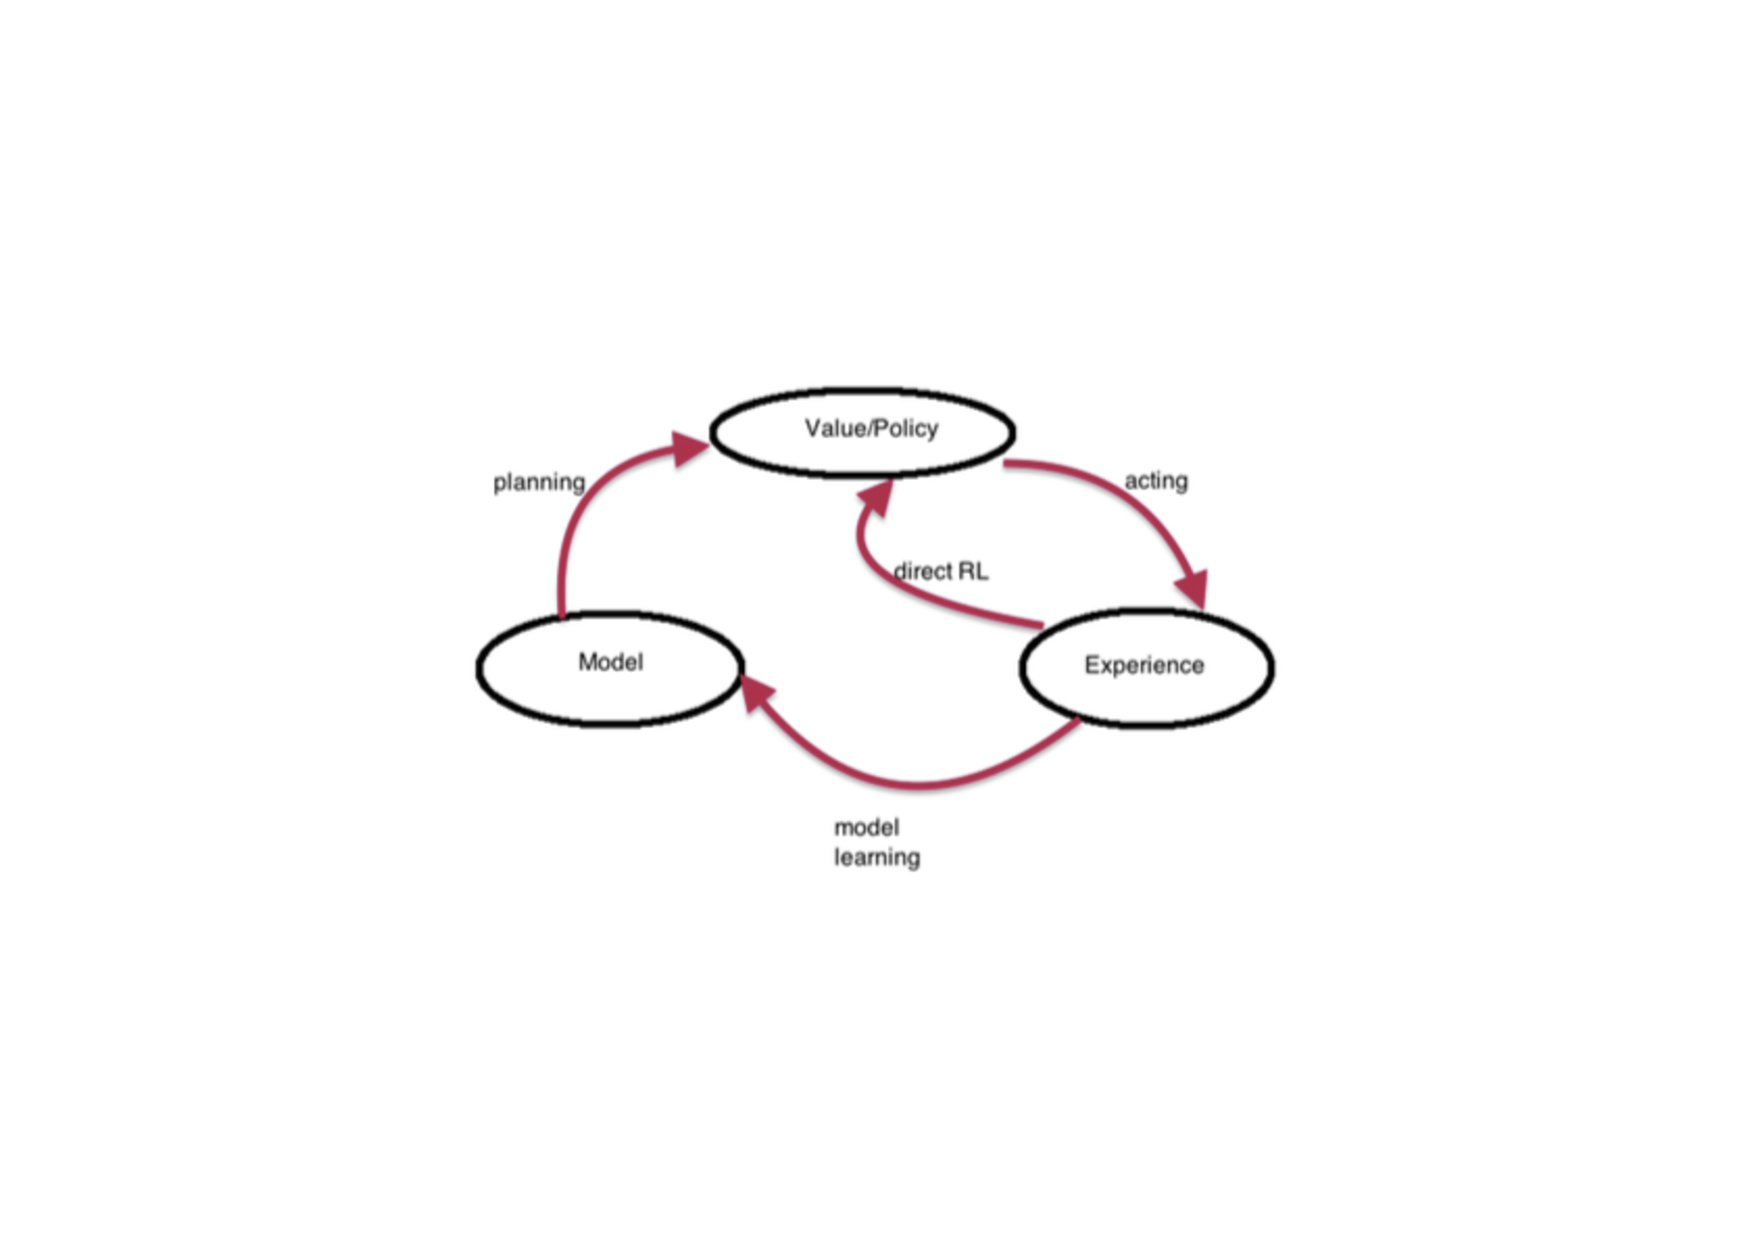
\includegraphics {dyna1}}
     \resizebox{75mm}{75mm} {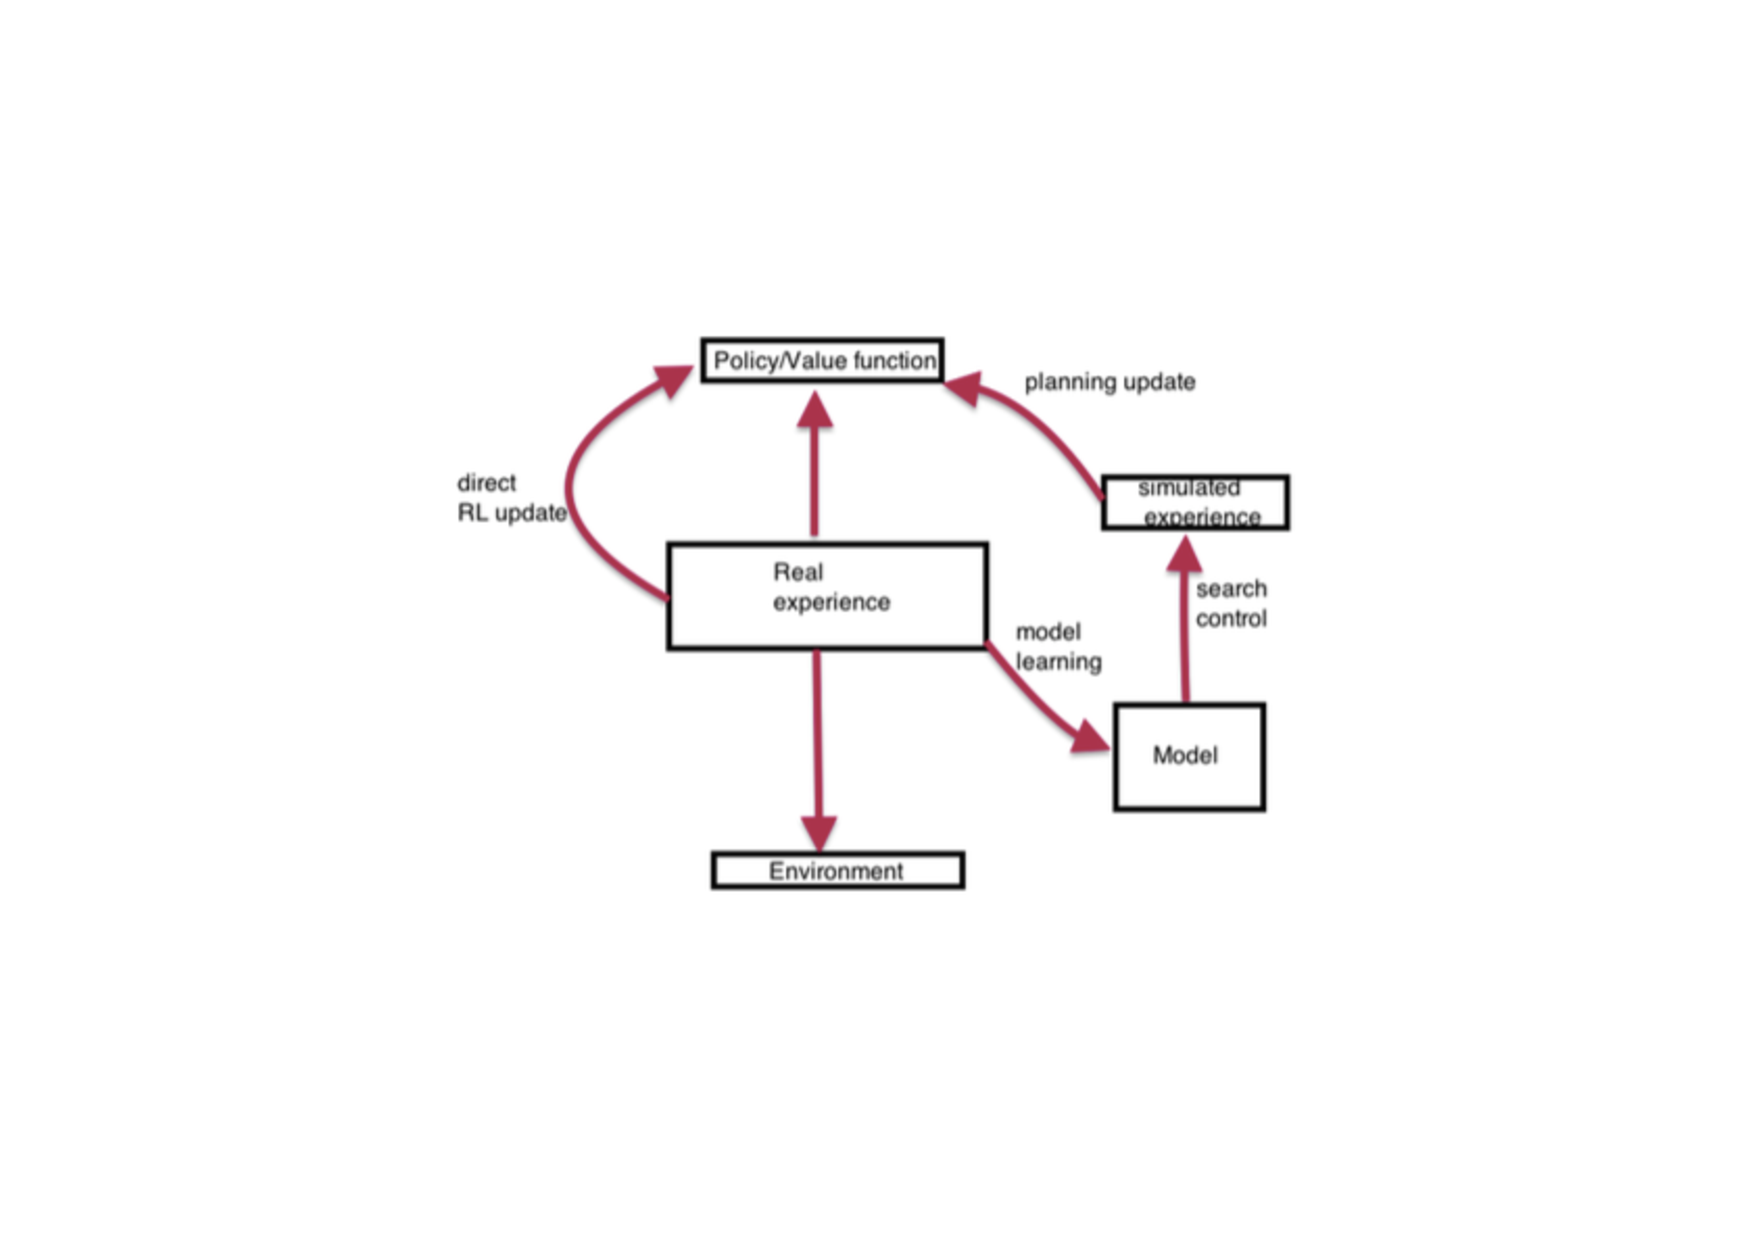
\includegraphics {dyna2}}
     \caption {Relationship between Value function , Experience and Models and DYNA framework}
   \label{fig:dyna}
   \end{center}
 \end{figure}
 

 
The real experience can be used to improve a model also known as model learning or improve the value function like in reinforcement learning, sometimes called direct reinforcement learning. In the \ref{fig:dyna} we summarized the possible relationship between experience, model learning and planning, direct reinforcement learning. It can be seen that experience can improve the value function both directly and indirectly. The indirect reinforcement learning stage is sometimes referred to as planning. These indirect methods are better in the sense that they make full use of experience and require fewer environmental interactions as planning is involved where as direct reinforcement learning is much simpler and are not affected if model is biased. DYNA framework brings together all the acting, model learning, planning and direct reinforcement learning into a single framework.

The \ref{fig:dyna} also shows how various stages interact with each other in the framework. The middle column represents the interaction between agent and environment. Left side represents the direct reinforcement learning update. In case of TD learning the value function update is the direct RL step.The right side corresponds to model based learning.An explicit model is maintained, in which each transaction is recorded. Planning takes place on learnt model using simulated experiences. For simulating experiences starting states and actions are selected using the model. We use search control to represent that in figure. Learning and planning are thus integrated in this common framework where learning is done on actual experience where as planning is done on simulated one which is based on model. The first 3 stages of acting, model learning and direct reinforcement learning are done in very small fraction of the time and planning is done in the rest of the time. An usual iteration of the agent would have it selecting an action to be performed in the current state based on some ε greedy approach. It then updates the value function and the transition is recorded in the model. Then N-iterations of planning take place on the existing transitions in the model. After each simulated transition, value function is updated which forms indirect RL update.

Improvements have been suggested to Dyna framework like Dyna+ where the most oldest action that has not been selected gets more reward. Other methods like prioritized sweeping makes sure that planning stage is more efficient. Selection of state during simulated experience is based on the value increment they offer.

We have seen that domain dependant heuristics in $RRT^*$ control the performance of the algorithm and efforts made to learn them using different methods \cite{perez12} . We would like to do TD learning on the trajectories to learn the appropriate value function across the state space. Also we have seen in \cite{svestrup10} where they represent the dynamic behaviour of the environment using some sort of cost fucntion across the state space with good results.In most of the real world problems it is critical to maintain the kino-dynamic constraints of the agent. We incorporate a local planner in the Extend step to take care of the kino-dynamic constraints when generating the RRT. We also would like to make the algorithm online by interleaving planning and acting. In \cite{dyna92} it was shown that DYNA framework beats other model free learning algorithms in sampling based MDP planning. With this motivation ,we propose an algorithm that implements policy iteration in continuous domains using RRTs and does replanning effectively using DYNA framework.  We first present the offline episodic version of the algorithm which computes path in less number of samples as it efficiently explores the state space and estimates the value function by planning using the current tree. 
\\
\\
\subsection{Algorithm}

\begin{algorithm}{DYNA-RRTPI(N)}{
\label{algo:DYNA-RRTPI}
\qcomment{Episodic offline version: builds RRT and implements policy iteration using DYNA framework}}
G$\leftarrow$ Build a vanilla RRT using Euclidean distance metric\\
$J_o \leftarrow$ NN-TD(G) i.e use the vanilla RRT over the space to initialize the J values\\ 
n $\leftarrow$ 0\\
\qwhile n $<$ N \\
$G_n \leftarrow$ Episode(S,$ || . ||_{J_{n-1}} $)\\
$J_n \leftarrow$ NN-TD($G_n$ , $J_{n-1})$ \\
n $\leftarrow$ n+1\qend\\
End of Algorithm
\end{algorithm}

\emph{Episode} procedure builds the RRT from start state to goal state using the value function and performs planning at every step.

\begin{algorithm}{Episode(S, $|| . ||_J$)}{
\label{algo:Dyna-Episode}
\qcomment{Build a RRT using value functions in dyna framework }}
 V(G) $\leftarrow$ {$x_{start}$};  E(G) $\leftarrow${$\phi$ } \\
\qwhile goal is not reached \\
$x_{rand}$ $\leftarrow$ Sample(S);\\
$x_{near}$ $\leftarrow$ Modified-Nearest($x_{rand}$, V(G) , $|| . ||_J $ );\\
$(x_{new}, a, r) \leftarrow$ Extend($x_{near}$, $x_{rand}$, S);\\
\qif Not-Colliding($x_{new}$, $x_{near}$,S)\\
\qthen Connect $x_{new}$ to $x_{near}$\\
V(G) $\leftarrow$ V(G) U {$ x_{new}$ }\\
E(G) $\leftarrow$ E(G) U ($x_{new}, a, r$)\\
$J(x_{near}) \leftarrow (1 - \alpha) J (x_{near} + \alpha (r + \gamma J(x_{new})))$ \qfi\\
J $\leftarrow$ RRT-Planning(G, J, number of iteration)\qend\\
return G\qend\\
End of Algorithm
\end{algorithm}
Steps 3,4,5 correspond to action selection in dyna framework. Steps 8,9 corresponds to model learning. Step 10 corresponds to direct RL update and step 11 is where planning is done. 

\begin{algorithm}{NN-TD(G, J)}{
\label{algo:NN-TD}
\qcomment{Estimates the value function J from the trajectories}}
Let $Y_n$ be the set of trajectories starting at $x_start$ till leaf nodes in G.\\
\qfor each trajectory $(s_o, a_o, r_1, s_1, a_1, r_2, s_2, ...)$ in $Y_n$\\
\qfor each pair $(s_i,a_i,r_{i+1}, s_{i+1})$\\
$J(s_i) = (1 - \alpha) J(s_i) + \alpha(r_i + \gamma J(s_{i+1})$\qrof\qrof\\
return J\\
End of Algorithm
\end{algorithm}

The basic nearest procedure in \ref{algo:Nearest} does not work well without proper initialization as lot of points tend to have same J value in the beginning. We modified the procedure to work with any intialization. We use euclidean distance to sort the points whose J values are close. This reduced the time taken to find the solution.

\begin{algorithm}{Modified-Nearest($x_{rand}$, V(G) , $|| . ||_J$ )}{
\label{algo: Modified-Nearest}
\qcomment{Finds a point nearest to given point in the graph with respect to the value function}}
 $X_{near} \leftarrow$ subset of vertices in V(G) such that  $x_{near} = \displaystyle arg\max_{x \in V(G)} (|| x - x_{rand}|| ) $\\
 return $x_{near} \in X_{near}$ that is closest to the goal when compared using euclidean distance\\
End of Algorithm
\end{algorithm}
$||x - y||_J$ = $J(x) - J(y)$ where x, y $\in$ S.
 
\begin{algorithm}{Extend($x_{near}$, $x_{rand}$, S)}{
\label{algo:Extend}
\qcomment{Finds a point close to $x_{rand}$ that is in $\epsilon-$neighbourhood of $x_{near}$} respecting the kinodynamic constraints}
 $x_{new} \leftarrow$  $\displaystyle arg\max_{a \in A} ||x - x_{rand} ||_J $|| $x_{new} - x_{near} ||$ is within kinematic bounds and action $a_{max}$ which generated $x_{new}$ is within the acceleration bounds\\
 $(r,x_{new} ) \leftarrow$ MDP($x_{near}$,a)\\ 
 return ($x_new, a, r$)\\
End of Algorithm
\end{algorithm}


\begin{algorithm}{RRT-Planning(G, $|| . ||_J$, number of iterations)}{
\label{algo:Simulate RRT sampling trajectories from given rrt and update value function}
\qcomment{samples trajectories using RRTs}}
n $\leftarrow$ 0\\
\qwhile n $<$ number of iterations\\
Randomly sample a point $x_{begin}$ from V(G)\\
Find a trajectory $Y$ with $x_{begin}$ as the root\\
\qfor each pair $(s_i,a_i,r_{i+1}, s_{i+1}) \in Y$\\
$J(s_i) = (1 - \alpha) J(s_i) + \alpha(r_i + \gamma J(s_{i+1})$\qrof\qend\\
return J\\
End of Algorithm
\end{algorithm}


For online algorithms it is not possible to predetermine paths by running multiple episodes. But DYNA-RRTPI will perform planning when the robot is executing the action. For online setting, the DYNA-RRTPI could be modified as

\begin{algorithm}{Online-DYNA-RRTPI( )}{
\label{algo:Online DYNA-RRTPI}
\qcomment{Online version: builds RRT and implements policy iteration using DYNA framework}}
G$\leftarrow$ Build a vanilla RRT using Euclidean distance metric\\
$J_o \leftarrow$ NN-TD(G) i.e use the vanilla RRT over the space to initialize the J values\\ 
\qwhile goal is not reached  \\
$x_{rand}$ $\leftarrow$ Sample(S);\\
$x_{near}$ $\leftarrow$ Nearest($x_{rand}$, V(G) , $|| . ||_J $ );\\
$(x_{new}, a, r) \leftarrow$ Extend($x_{near}$, $x_{rand}$, S);\\
\qif Not-Colliding($x_{new}$, $x_{near}$,S)\\
\qthen Connect $x_{new}$ to $x_{near}$\\
V(G) $\leftarrow$ V(G) U {$ x_{new}$ }\\
E(G) $\leftarrow$ E(G) U ($x_{new}, a, r$)\\
$J(x_{near}) \leftarrow (1 - \alpha) J (x_{near} + \alpha (r + \gamma J(x_{new})))$ \qfi\\
J $\leftarrow$ RRT-Planning(G, J, number of iteration)\qend\\
End of Algorithm
\end{algorithm}

Number of iterations of planning could be modified as per the time available for planning during the execution phase of robot.  Another important parameter to take care of is $\alpha$ which should typically be very small in stochastic environments for the value function to converge. $\gamma$ value is domain dependant.  The algorithm gradually builds a tree from the start to goal states in an online fashion. It uses  RRT-based planning to improve the value function estimates by using the model already learnt. Even if dynamic environments the algorithm works well because the value function adapts to the moving environment at every time step and hence the around the obstacles the value function gives unfavourable values and guides the tree towards higher value goal regions. 

If the environment has undergone drastic changes where replanning is required DYNA-RRTPI could be easily modified to include replanning efficiently. The modified algorithm is given as follows.

\begin{algorithm}{Replan-DYNA-RRTPI( )}{
\label{algo:Replan-DYNA-RRTPI}
\qcomment{Online version: builds RRT and implements policy iteration using DYNA framework}}
G$\leftarrow$ Build a vanilla RRT using Euclidean distance metric\\
F $\leftarrow$ initialize to empty set of forest of disconnected trees.
$J_o \leftarrow$ NN-TD(G) i.e use the vanilla RRT over the space to initialize the J values\\ 
\qwhile Graph G doesnt contain goal \\
\qif Graph is not empty \\
\qthen Prune(G,F)\\
\qelse Intialize V(G) $\leftarrow$ $\{x_{start} \}$\qfi\\
$x_{rand}$ $\leftarrow$ Modified-Sample(S,F);\\
$x_{near}$ $\leftarrow$ Modified-Nearest($x_{rand}$, V(G) , $|| . ||_J $ );\\
$(x_{new}, a, r) \leftarrow$ Extend($x_{near}$, $x_{rand}$, S);\\
\qif Not-Colliding($x_{new}$, $x_{near}$,S)\\
\qthen Connect $x_{new}$ to $x_{near}$\\
V(G) $\leftarrow$ V(G) U {$ x_{new}$ }\\
E(G) $\leftarrow$ E(G) U ($x_{new}, a, r$)\\
$J(x_{near}) \leftarrow (1 - \alpha) J (x_{near} + \alpha (r + \gamma J(x_{new})))$ \qfi\\
J $\leftarrow$ RRT-Planning(G, J, number of iteration)\qend\\
End of Algorithm
\end{algorithm}

\begin{algorithm}{Prune(Graph G, Forest F)}{
\label{algo:Prune}
\qcomment{Perfoms collision checks on all nodes and removes nodes that are not in $C_{free}$}}
\qfor each node q $\in$ V(G) and F\\
\qif Not-valid (q)\\
\qthen remove q from G and F\\
split the tree at q and add subtrees to F\qfi\qrof\\
\qif G is empty \\
\qthen Initialize G and add $x_{start}$ to V(G)\qfi\\
End of Algorithm
\end{algorithm}

\begin{algorithm}{Modified-Sample(S,F)}{
\label{algo: Modified-Sample}
\qcomment{Returns a point to which the RRT would try to expand to}}
prob $\leftarrow$ Random(0,1)\\
\qif prob $<$ $p_{goal}$\\
\qthen $x_{result}$ $\leftarrow$ $x_{goal}$\\
\qelse \qif prob $< p_{goal} + p_{forest}$\\
\qthen $x_{result} \leftarrow$ root of a randomly sampled tree from $F$ , the forest of disconnected trees.\\
\qelse $x_{result}$ $\leftarrow$ Randomly sample a point from the state space \qfi\qfi\\
return $x_{result}$\\
End of Algorithm
\end{algorithm}

The above modification to the regular DYNA-RRTPI would use the previous successful trees regrow the trees at each instant. For every time step , the tree is inspected for any nodes in $C_{forbidden}$ and if it finds such nodes, the algorithm breaks the tree at that node and places the subtrees in the Forest F which would be used later on for sampling for points to extend the RRT. The algorithm for replanning can be made similar to both ERRT \cite{errt} or DRRT \cite{drrt} based on the choice of parameter $p_{forest}$. In pruning stage if we maintain just a single tree instead of a forest of disconnected trees we would essentially get an analogue of ERRT where when selecting a node in \textit{Modified-Sample} procedure we would have sampled a node from the single saved trajectory or waypoint cache we stored in pruning stage. The algorithm could be modified into an analogue of DRRT if instead of storing both the sub trees in pruning stage, we throw away the tree that is not connected to the start state. Hence in that case we would have to regrow from that sub-tree which is still connected to the start state. The suggested algorithm has the good properties of both ERRT and DRRT performs better that both ERRT and DRRT in replanning tasks \cite{mprrt}

\section{Experiments}

We evaluated our algorithm on discrete and continuous domains. For discrete domain we used a 15x15 grid world with obstacles in some grids. The action space included moving in either top, left, right, down directions.

 \begin{figure}[htpb]
   \begin{center}
     \resizebox{130mm}{80mm} {\includegraphics *{gridworlddomain}}
     \caption { 15x15 grid world domain with goal and obstacles. Start state is in cell (1,4) and goal is in (11,11) cell}
     \end{center}
     \end{figure}
     
	Our algorithm is run for 100 episodes with maximum of 200 iterations per episode. For planning in each step we allowed a maximum of 50 iterations. We used ( state,action) value funcion for estimating the node to expand to. The algorithm learnt the optimal policy of 17 cell path in - episodes. We compare it with RRTPI algorithm which is run without planning step. Initially we ran it without compensating for the extra planning DYNA-RRTPI is doing. We ran with compensation also. RRTPI too learnt the optimal policy in almost same number of iterations as our algorithm. The alpha value choosen was 0.1 for this setting. 
	
	 \begin{figure}[htpb]
   \begin{center}
     \resizebox{140mm}{140mm} {\includegraphics *{discrete}}
     \caption { Number of iterations to reach goal vs Episode for DYNA-RRTPI and RRTPI}
     \end{center}
     \end{figure}
     
For continuous domain, we ran RRTPI algorithm on 2-D continuous rectangular state space spanning from (0,0) to (100,100) by initializing the value function uniformly. We limited the step length RRTPI can take in each time step. The start point is at (50,50) and goal is to reach to top of (95,95). Transitions that above (95,95) give reward of 100 and no reward otherwise.
 
  \begin{figure}[htpb]
   \begin{center}
     \resizebox{120mm}{100mm} {\includegraphics *{rrtpi_uniformly}}
     \caption {Value function initialized uniformly, Start point at (50,50) , goal at (95,95)}. 
     \label{rrt-notworking}
     \end{center}
     \end{figure}
 
Value of a new state is apporimated using the value of the k-nearest neighbours which are already visited. Since most of the points have same value function a tree was not being generated towards the goal as seen in \ref{rrt-notworking}. Hence we first grew plain RRT based on eucliean distance and used our value estimation prodecure \ref{algo:NN-TD} to initialise the value function. Then RRT grew towards the goal as seen in \ref{rrt-working}. We also added a little bias towards the goal to make the RRT reach goal faster. Also we included ranking based on euclidean closeness to the goal when value estimates of the points are same. This also helped in guiding the RRT towards goal.




\begin{figure}[htpb]
   \begin{center}
     \resizebox{120mm}{100mm} {\includegraphics *{rrtpi_withrrt}}
     \caption {Value function initialized using plain RRT, Start point at (50,50) , goal at (95,95)}. 
     \label{rrt-working}
     \end{center}
     \end{figure}

We ran experiments in puddle world domain where transitions through puddles are allowed but are negatively rewarded and the negative reward is proportional to how deep inside the puddle the agent is.. We  used the concept of canonical trajectories proposed by Fraichard \cite{fraichard99}. Canonical trajectories follow discrete and piecewise constant acceleration for the agent. We also set bounds on velocity of the agent and the rate of change of velocity is also bounded. All these were taken care of by the local planner which only extends to points which it can reach with in these kino-dynamic constraints. 


\begin{figure}[htpb]
   \begin{center}
     \resizebox{140mm}{70mm} {\includegraphics *{continuouspuddleworld}}
     \caption {DYNARRTPI vs RRTPI in 2-D continuous puddle world from (0,0) to (50,50) with puddle of radius 5 at (30,10) }. 
     \label{continuouspuddleworld}
     \end{center}
     \end{figure}

In the experiment we did, RRTPI found solutions initially due to randomness inherent to the algorithm. The number of steps taken to find goal reduced after 20 episodes. Each episode of RRTPI has been run to a maximum of 200 iterations. In \ref{continuouspuddleworld}. The blue curve going out of figure around 5 episodes indicates that it did not find a solution for that episode. DYNA with 40 planning iterations per RRT iteration found solutions in less number of steps even in the initial episodes. In this task the value functions distribution across the domain for both the algorithms can be seen in \ref{puddleworldvalue}. If the $\alpha$ is too low then the RRT is not guided towards the goal and learning takes long times as direction towards goal is not captured in the value function. It can be seen in \ref{rrrtpilowalpha}


\begin{figure}[htpb]
   \begin{center}
     \resizebox{75mm}{75mm} {\includegraphics *{dyna3}}
      \resizebox{75mm}{75mm} {\includegraphics *{rrtpi40}}
     \caption { The value function distribution for the puddle world task. The region in pink is where value function is positive, yellow represents the neutral region where as black represents the region where the value function is negative. The green line is the path learnt in RRT grown in that episode. The left graph is for 3 episodes of DYNA-RRTPI and right graph for RRTPI.}. 
     \label{puddleworldvalue}
     \end{center}
     \end{figure}
 
\begin{figure}[htpb]
   \begin{center}
     \resizebox{75mm}{75mm} {\includegraphics *{rrtpidivergingatlowalpha}}
     \caption {RRTPI not reaching towards the goal at very low alpha }. 
     \label{rrrtpilowalpha}
     \end{center}
     \end{figure}
     
 
 
 
 We set up two puddles in the domain and shifted our start state away from the puddles and goal so that puddles would come in the direct path from start to goal and ran RRTPI with the modification we proposed above. We initialized the value function using a vanilla RRT with euclidean distance and used nearest neighbour TD(0) method to learn the values from the sampled trajectories. It can be seen in \ref{rrtwithourchanges} where each image represent a snapshot of the RRT after each episode, the  top left is the initial RRT which is run to initialize the value function. It has no knowledge of the puddles. In the later images the regions are color coded for better representation. Area with pink points represent the region where value function is positive and are with black dots represent negative value function region and yellow stands for value function which is close ro zero. The two blue circles are the puddles. $\alpha$ value is set to 0.1 to begin with. We can see that it learns a path in the first episode the green path represent a path taken while running RRTPI. Episode ends when a path is found. It has not explored the state space completely, hence it tries to explore other regions also in the later iteratons. In middle right image it can be seen that RRT initially ventures into unknown second puddle for the entire episode as the value updates are only done at the end of episode. It could not correct the path until the start of the next episode. This is one drawback of not having a planning procedure unlike our algorithm \ref{algo:DYNA-RRTPI} where after each iteration a planning stage takes place. In the next episode RRTPI corrects its path and assigns negative value functions to areas near the second puddle also. It can also be seen that high resolution sampling is done closer to goal and it learns a trajectory from the start point to goal point. This run clearly demonstrates the disadvantage of RRTPI where update to value function is done only at the end of the episode and in our method DYNA-RRTPI after each iteration planning takes place and thus it can run in online setting also.

\begin{figure}[htpb]
   \begin{center}
     \resizebox{160mm}{150mm} {\includegraphics *{rrtrun0}}
      \resizebox{150mm}{75mm} {\includegraphics *{rrtrun2}}
     \caption { A run of RRTPI with the modifications we proposed. }. 
     \label{rrtwithourchanges}
     \end{center}
     \end{figure}

We tested the effectiveness of both algorithms in dynamic setting. We leant the value function in a scenario and incresed the puddle radius and saw how both algorithms respond to the changes in enironment. For the change we made i.e increase of puddle radius from 2 to 5 units where now puddle takes a considerable portion in the direct path from start to goal as seen in the figure , RRTPI took 10 episodes of each 200 maximum iterations to again to form proper plans, where as our algorithm DYNA-RRTPI  responded to the changes in the same episode itself. It is also intuitive that RRTPI would not learn the changes immediately as the value function updates are done only at the end of the episode and we can expect considerable amount of updates only if a good portion of the changed space is covered by the newly sampled trajectory. \\ \\

\begin{figure}[htpb]
   \begin{center}
     \resizebox{50mm}{50mm} {\includegraphics *{dynabeforechange}}
      \resizebox{50mm}{50mm} {\includegraphics *{dynaafterchange}}
     \caption { DYNA-RRTPI in successive episodes when puddle radius is increased. }. 
     \label{dynapuddlemove}
     \end{center}
     \end{figure}

\begin{figure}[htpb]
   \begin{center}
     \resizebox{50mm}{50mm} {\includegraphics *{rrtpibeforechange}}
      \resizebox{50mm}{50mm} {\includegraphics *{rrtpiafterchange}}
       \resizebox{50mm}{50mm} {\includegraphics *{rrtpiafter10episodes}}
     \caption {from left to right, RRTPI before puddle expansion, RRTPI in the episode after puddle expansion and RRTPI after 10 episodes }. 
     \label{dynapuddlemove}
     \end{center}
     \end{figure}

The agent under our algorithm is reactive and always deliberative, responding instantly to the updates in environment when latest sensory information is given to it because of the planning step involved in every iteration. Hence it can be applied to dynamic environments in online setting.
 
 
\chapter{Conclusion and Future Work}
We introduced a way of learning optimal solutions to motion planning problem in unknown non-stationary environments using DYNA and efficient replanning techniques. We assume just a minimum generative model which would tell if a given state is in $C_{free}$ or not. Our algorithm builds a near optimal RRT in the state space with the learnt value function in continous state spaces. We have presented episodic, offline and online versions of our algorithm. We have showed use of nearest neighbour methods for tackling the value evaluation in continuous state space. We implemented our algorithm on continuous puddle world domain for an agent follwing kino-dynamic constraints using a local planner in the extend step of growing RRT. Our algorithm DYNA-RRTPI integrates good sampling based planning techniques into a framework interleaving directRL updates, model building and planning and thus solving problems in dynamic continuous unknown environments with efficient replanning techniques follwing kino-dynamic contraints of the agent and the environment. In future instead of simulatons, we can apply our algorithm to dynamic real world 2-D robot navigation and a high dimensional non-holonomic arm navigation tasks and compare it against the state of the art methods like $RRT^*$. 


%%%%%%%%%%%%%%%%%%%%%%%%%%%%%%%%%%%%%%%%%%%%%%%%%%%%%%%%%%%%
% Appendices.
%\appendix
%\chapter{Appendix}
%\input{appendix.tex}
% Bibliography.
%\pagebreak
%\begin{singlespace}
%  \begin{small}
%	\bibliography{D59} E. Dijkstra. A note on two problems in connexion with graphs. Numerische Mathe- matik, 1:269–271, 1959.
%  \end{small}
%\end{singlespace}

\begin{thebibliography}{99}
\bibitem{d59}
	E. Dijkstra, 
  \emph{A note on two problems in connection with graphs},
	Numerische Mathematik,
  1959.

\bibitem{hnb68}
	P. Hart, N. Nilsson, and B. Rafael, 
  \emph{A formal basis for the heuristic determination of minimum cost paths},
	IEEE Transactions on Systems Science and Cybernetics, 4:100107,
	 1968.


\bibitem{choset05}
	H. Choset, K. Lynch, S. Hutchinson, G. Kantor, W. Burgard, L. Kavraki, and S. Thrun,
  \emph{Principles of Robot Motion: Theory, Algorithms, and Implementations},
	MIT Press, Cambridge, MA,
	 2005.
	 
\bibitem{deberg00}
 M.deBerg,M.vanKreveld,M.Overmars,and O.Schwarzkopf ,
  \emph{ComputationalGeom- etry: Algorithms and Applications},
	Springer-Verlag, Heidelberg, Germany, 2nd edition
	 2000.

\bibitem{latombe91}
	J. Latombe,
  \emph{Robot Motion Planning},
	Kluwer Academic Publishers, Boston, MA,
	 1991.
	 
 \bibitem{lav06}
	S.LaValle,
  \emph{PlanningAlgorithms},
	Cambridge University Press, New York,
	 2006.

 \bibitem{perez79}
	Tomás Lozano-Pérez and Michael A. Wesley,
  \emph{An algorithm for planning collision-free paths among polyhedral obstacles},
	Commun. ACM 22, 10, 560-570,
	 1979.

 \bibitem{canny88}
  J.Canny,
  \emph{MIT Press, Cambridge, MA},
	MIT Press, Cambridge, MA,
	 1988.

 \bibitem{schsha83}
	J. Schwartz and M. Sharir,
  \emph{On the piano movers’ problem: I. The case of a two-dimensional rigid polygonal body moving amidst polygonal barriers},
	Communications on Pure and Applied Mathematics, 36:345–398,
	 1983.

 \bibitem{reif79}
	J.Reif,
  \emph{Complexity of the mover’s problem and generalizations},
	 In Proc. IEEE Symp. on Foundations of Computer Science, pages 421–427,
	 1979.


 \bibitem{stentz95}
	A. Stentz,
  \emph{The focussed D* algorithm for real-time replanning},
	 Proceedings of the International Joint Conference on Artificial Intelligence, pp. 1652–1659,
	 1995.

 \bibitem{koeni02}
	S.Koenigand, M.Likhachev,
  \emph{D*Lite},
	 In Proceedings of the National Conference on Artificial Intelligence (AAAI),
	 2002.

%quadtrees 
 \bibitem{samet88}
	H. Samet,
  \emph{An Overview of Quadtrees, Octrees, and Related Hierarchical
Data Structures},
	 NATO ASI Series, Vol. F40,
	 1988.
	 
	 %D*
	  \bibitem{stentz94}
	Stentz, Anthony,
  \emph{Optimal and Efficient Path Planning for Partially-Known Environments},
	Proceedings of the International Conference on Robotics and Automation: 3310–3317,
	 1994.
	 
	 
 \bibitem{hr07}
	Eric A. Hansen, Rong Zhou,
  \emph{Anytimre A* Anytime heuristic search},
	 Journal of Artificial Intelligence Research - JAIR ,
	 2007.
	 
%A*	 
	  \bibitem{hnr68}
	Hart, P., Nilsson, N., Raphael, B,
  \emph{A formal basis for the heuristic determination of
minimum cost paths},
	 IEEE Transactions on Systems Science and Cybernetics (SSC),
4 (2), 100–107,
	 1968.	 
	 

 %visibility graphs
	  \bibitem{visgraph00}
	de Berg Mark, van Kreveld Marc, Overmars Mark, Schwarzkopf, Otfried,
  \emph{Chapter 15: Visibility Graphs},
	 Computational Geometry (2nd ed.), Springer-Verlag, pp. 307–317,
	 2000.	 
	 

%arf	 
	  \bibitem{khatib86}
	O. Khatib,
  \emph{Real-time obstacle avoidance for manipulators and mobile robots},
	 International Journal of Robotics Research, 5(1):90–98,
	 1986.	 



%practical arf
	  \bibitem{gecui02}
	S.S. Ge, Y.J. Cui,
  \emph{Dynamic Motion Planning for Mobile Robots Using Potential Field Method},
	Autonomous Robots, Volume 13, Issue 3, pp 207-222 November,
	 2002.	 

%practical arf
	  \bibitem{barra91}
	J. Barraquand and J. Latombe,
  \emph{Robot motion planning: a distributed representation approach},
	International Journal of Robotics Research, 10(6):628649,
	1991.	 


%rrt-star and prm-star
	  \bibitem{karaman11}
	Sertac Karaman and Emilio Frazzoli ,
  \emph{Sampling-based algorithms for optimal motion planning},
	International Journal of Robotics Research, June , 846-894,
	2011.	 

 %prob comp prm
	  \bibitem{kavraki98}
	L. E. Kavraki, M. N. Kolountzakis, and J. C. Latombe,
  \emph{Analysis of probabilistic roadmaps for path planning},
	IEEE Transactions on Roborics and Automation, 14(1):166-171,
	1998.	 
	
%lavalle 2006
	  \bibitem{lav06}
	S. M. LaValle,
  \emph{Planning Algorithms},
	Cambridge University Press,
	2006.	 


%prm
	  \bibitem{kavraki96}
	L. E. Kavraki, P. Svestka, J. C. Latombe, and M. H. Overmars.,
  \emph{Probabilistic roadmaps for path planning in high-dimensional configuration spaces},
	IEEE Transactions on Robotics and Automation, 12(4):566-580,
	1996.	 

%practical arf
	  \bibitem{linde05}
	S. R. Lindemann and S. M. LaValle ,
  \emph{Current issues in sampling-based motion planning},
	In P. Dario and R. Chatila, editors, Eleventh International Symposium on Robotics Research, pages 36-54. Springer,
	2005.	 

	  \bibitem{lav01}
	Steven M. Lavalle and James J. Kuffner ,
  \emph{Rapidly-exploring Random Trees: Progress and prospects},
	 Algorithmic and Computational Robotics: New Directions, pp. 293-308,
	2001.	 
	
	  \bibitem{bruce02}
	J. Bruce and M. Veloso,
  \emph{Real-time randomized path planning for robot navigation},
	in Proceedings of the IEEE International Conference on Intelligent Robots and Systems (IROS),
	2002.	 
	
	  \bibitem{kuffner03}
	J. Kuffner, K. Nishiwaki, S. Kagami, M. Inaba, and H. Inoue,
  \emph{Motion planning for humanoid robots},
	in Proceedings of the International Symposium on Robotics Research (ISRR),
	2003.	 
	

	  \bibitem{kim03}
	J. Kim and J. Ostrowski,
  \emph{Motion planning of aerial robots using Rapidly-exploring Random Trees with dynamic constraints},
	in Proceedings of the IEEE International Conference on Robotics and Automation (ICRA)
	2003.	 
	

	  \bibitem{oriolo04}
	 G. Oriolo, M. Vendittelli, L. Freda, and G. Troso,
  \emph{The SRT Method: Randomized strategies for exploration},
	in Proceedings of the IEEE International Conference on Robotics and Automation (ICRA),
	2004.	 


 \bibitem{kuffner00}
	 James J. Kuffner Jr. , Steven M. Lavalle ,
  \emph{RRT-Connect: An efficient approach to single-query path planning},
	in Proceedings of the IEEE International Conference on Robotics and Automation (ICRA),
	2000.	

 \bibitem{brooks09}
	 A. Brooks, T. Kaupp, and A. Makarenko,
  \emph{Randomised mpc-based motion-planning for mobile robot obstacle avoidance,},
	in Proceedings of the IEEE International Conference on Robotics and Automation (ICRA),
	2009.	

 \bibitem{shkolnik09}
	 A. Shkolnik, M. Walter, and R. Tedrake,
  \emph{Reachability guided sampling for planning under differential constraints},
	in Proceedings of the IEEE International Conference on Robotics and Automation (ICRA),
	2009.	

 \bibitem{ferguson07}
	D. Ferguson and A. Stentz,
  \emph{Anytime, dynamic planning in high- dimensional search spaces},
	in Proceedings of the IEEE International Conference on Robotics and Automation (ICRA),
	2007.	
	

 \bibitem{yasin10}
	Yasin Abbasi-Yadkori, Joseph Modayil and Csaba Szepesvari,
  \emph{Extending Rapidly-Exploring Random Trees for Asymptotically Optimal Anytime Motion Planning},
	IEEE/RSJ International Conference on Intelligent Robots and Systems,
	2010.	

 \bibitem{perez12}
	A. Perez, R. Platt, G. Konidaris, L. Kaelbling, and T. Lozano Perez,
  \emph{LQR-RRT : Optimal sampling-based motion planning with automatically derived extension heuristics},
	in Proceedings of the IEEE International Conference on Robotics and Automation,
	2012.	
	
	
	
	
	
Fraichard. Trajectory planning in a dynamic workspace: a ‘state-time’ approach. Advanced Robotics, 13(1):75–94, 1999.

  \bibitem{fraichard99}
	Fraichard,
  \emph{Trajectory planning in a dynamic workspace: a ‘state-time’ approach},
	dvanced Robotics, 13(1):75–94, 
	1999.
	
J. van den Berg and M. Overmars. Roadmap-based motion planning in dynamic environments. IEEE Transactions on Robotics, 21(5):885–897, 2005 
 \bibitem{jm05}
	J. van den Berg and M. Overmars,
  \emph{Roadmap-based motion planning in dynamic environments. IEEE Transactions on Robotics},
	 IEEE Transactions on Robotics, 21(5):885–897, 
	 2005.
	 
	 
 \bibitem{svestrup10}
	Aalborg Universitet , Mikael Bak , Thomas Andersen , Hans Jørgen , Mikael Svenstrup , Thomas Bak , Hans Jørgen Andersen,
  \emph{Trajectory Planning for Robots in Dynamic Human Environments},
	IEEE/RSJ International Conference on Intelligent Robots and Systems (IROS), 
	2010.
	
 \bibitem{dyna92}
	Richard S. Sutton,
  \emph{Reinforcement Learning Architectures},
	Proceedings of International Symposium on Neural Information Processing , 
	1992.
	
 \bibitem{aoude13}
	Georges S. Aoude, Brandon D. Luders, Joshua M. Joseph, Nicholas Roy, Jonathan P. How,
  \emph{Probabilistically safe motion planning to avoid dynamic obstacles with uncertain motion patterns},
	Autonomous Robots
	July Volume 35, Issue 1, pp 51-76,
	2013.	
	

 \bibitem{aoude10}
	Aoude GS, Luders BD, How JP,
  \emph{Sampling-based threat assessment algorithms for intersection collisions involving errant drivers},
	in IFAC Symposium on Intelligent Autonomous Vehicles, Lecce, Italy,
	2010.	
	
 \bibitem{kutawa08}
	Yoshiaki Kuwata, Gaston A. Fiore, Justin Teo, Emilio Frazzoli, Jonathan P. How,
  \emph{Motion Planning for Urban Driving using RRT},
	In Proceedings of the IEEE/RSJ International Conference on Intelligent Robots and Systems , 
	2008.
	
	 \bibitem{fulgenzi08}
	Fulgenzi C, Tay C, Spalanzani A, Laugier C,
  \emph{Probabilistic navigation in dynamic environment using rapidly-exploring random trees and gaussian processes},
	in: IEEE/RSJ International Conference on Intelligent Robots and Systems (IROS), Nice, France, pp 1056–1062
	2008.	
	
 \bibitem{errt}
	J. Bruce and M. Veloso,
  \emph{Real-time randomized path planning for robot navigation},
	in Proceedings of IROS-2002, Switzerland, October 2002, an earlier version of this paper appears in the Proceedings of the RoboCup-2002 Symposium.
	
 \bibitem{drrt}
	D. Ferguson, N. Kalra, and A. Stentz,
  \emph{Replanning with RRTs},
	in Proc. IEEE International Conference on Robotics and Automation ICRA ,
	 2006. 
	 
 \bibitem{mprrt}
	M. Zucker, J. Kuffner, and M. Branicky,
  \emph{Multipartite rrts for rapid replanning in dynamic environments},
	in Proc. IEEE International Conference on Robotics and Automation (ICRA) pp. 1603–1609 , 
	2007.


 \bibitem{lav02}
	S. M. Lavalle,
  \emph{From dynamic programming to RRTs: Algorithmic design of feasible trajectories},
	in Control Problems in Robotics, Springer-Verlag,
 2002.
 
 (R.S. Sutton and A.G. Barto. Reinforcement learning: An introduction, volume 28. MIT press, 1998.) 
 \bibitem{rltextbook}
	R.S. Sutton and A.G. Barto,
  \emph{Reinforcement learning: An introduction},
	volume 28. MIT press, 
	1998.
 
 (R. S. Sutton. “Learning to predict by the methods of temporal differences”. Machine Learning, 3, 1988.)
 \bibitem{tdlearning}
	R. S. Sutton,
  \emph{Learning to predict by the methods of temporal differences},
	Machine Learning, 3, 
	1988.
	
	 \bibitem{thrun93}
	Sebastian Thrun and Anton Schwartz,
  \emph{Issues in Using Function Approximation for Reinforcement Learning},
	in Proceedings of the Fourth Connectionist Models Summer School, Lawrence Erlbaum Publisher, Hillsdale, NJ, Dec,
	1993.
	
\bibitem{neumann07}
	Gerhard Neumann, Michael Pfeiffer, Wolfgang Maass,
  \emph{Efficient Continuous-Time Reinforcement Learning with Adaptive State Graphs},
	Machine Learning: ECML 2007, Lecture Notes in Computer Science Volume 4701, 2007, pp 250-261.



\bibitem{rrtpi}
	Manimaran, S. S., and Ravindran, B.,
  \emph{RRTPI: Policy Iteration on Continuous Domains using Rapidly-exploring Random Trees},
	 In the Proceedings of the IEEE International Conference on Robotics and Automation (ICRA 2014), pp. 4362-4367. Hong Kong, China. IEEE Press.
\end{thebibliography}

%%%%%%%%%%%%%%%%%%%%%%%%%%%%%%%%%%%%%%%%%%%%%%%%%%%%%%%%%%%%

\end{document}